\chapterimage{capitulos/informatica/imagenes/cover}
\chapterimagedescription{Placa base de una computadora con sus circuitos impresos}
\chapterimageauthor{Fotografía de Blickpixel}

\chapter{Informática}
\index{Informatica@Informática}

En este capítulo veremos como los conceptos del capítulo anterior se aplican a
los conceptos que utilizamos día a día como usuarios de computadoras.
Veremos qué son los archivos, las carpetas y los programas, y veremos como se
crean los programas utilizando lenguajes de programación.

Esto nos llevará a analizar qué es exactamente un lenguaje y a ver diversos tipos
de lenguajes que existen en informática. Nos centraremos luego en los lenguajes
de marcado, como una forma de representar datos mediante texto.

\section{Archivos y extensiones}

Cuando utilizamos la computadora sabemos bien donde está guardada nuestra información.
Archivos, ubicados en carpetas como ``Mis Documentos'' poseen nuestros documentos
de texto y planillas de cálculo. Otros, ubicados en ``Mis Imágenes'' mantienen
nuestros recuerdos en forma de imágenes digitales.

Pero ¿Qué es exactamente un archivo informático? ¿Y qué es un directorio?
En esta sección analizaremos esas preguntas desde dos puntos de vista. En
una primer instancia, lo veremos desde el punto de vista de la computadora
en bajo nivel. Luego, veremos cuales son los detalles importantes desde el punto
de vista del usuario final para poder administrar y manejar mejor los archivos.

También analizaremos diversos tipos de archivos, y veremos como el sistema es
capaz de identificar esos tipos de archivos, y como opera con y sobre ellos.

\subsection{Archivos informáticos}
\index{Archivos Informaticos@Archivos Informáticos}

Un archivo informático no es más que la representación digital de un archivo
físico que se tiene en papel. Puede contener texto, imágenes, videos, modelos
tridimensionales, o cualquier otro contenido que uno quiera almacenar y
manipular en la computadora.

En última instancia, un archivo informático se reduce solo a una serie de bits que la
computadora es capaz de almacenar, transmitir, y manipular mediante los circuitos
que posee, como ya mencionamos previamente. Pero surge la pregunta: ``¿Qué es lo
que hace que una serie de ceros y unos sea una imagen, y otra sea un video, audio
o un modelo 3D?''. La respuesta radica en el \textbf{formato de archivo}.

\index{Formato}
\textbf{Cada archivo tiene un formato, que es lo que determina como la computadora
debe leer e interpretar los bits que componen al mismo.} El formato
está relacionado a la codificación que se haya elegido. Por ejemplo, la
codificación que elegimos para las imágenes en la sección anterior, es una, de
muchas posibles codificaciones.

\textbf{No hay un único formato para cada tipo de archivo}, por ejemplo, no hay
un único formato para todo lo que son imágenes. Cada formato tiene sus ventajas
y desventajas, y está pensado para solucionar problemas puntuales que tienen
que ver con representar ese archivo en la computadora en alguna forma particular,
por ejemplo, con mayor calidad, con menor espacio posible, etc.

La información se \textbf{codifica} como binario y se \textbf{decodifíca} como
información (de binario a información). Esa interpretación de los datos en ida y
vuelta está dada entonces por el \textbf{formato de archivo}. Para que los
archivos puedan compartirse y leerse como se espera por cualquier computadora,
la forma en la que interpretamos esos ceros y unos debe ser la misma para todos,
por lo que los formatos están \textbf{estandarizados}.

\begin{definition}\index{Archivo}
    Un \textbf{archivo informático} es la representación digital de un archivo
    físico, el cuál se encuentra almacenado en un dispositivo de almacenamiento
    como una cadena de bits la cual es la codificación de lo representado utilizando
    algún código determinado, determinando su formato. Un archivo además tiene un
    nombre y un tamaño (que depende de la cantidad de bits que tiene el archivo).\autocite[vid. p.13]{gookin_2005}
\end{definition}

Para tener una mejor idea, analicemos un ejemplo simple. Una fotografía o imagen
digital puede almacenarse en alguno de los muchos formatos disponibles para ello.
Tres de los más utilizados son los formatos RAW, JPEG y PNG.
\begin{itemize}
    \item Las imágenes en formato RAW son aquellas en donde se almacena toda la
        información para cada pixel de la imagen. Es decir, se divide la imagen
        en una grilla gigante de pequeños puntos (pixeles), y el archivo consiste
        en la información de que color debe tener cada pixel. Esto otorga la
        mejor precisión de los colores y la mejor calidad de imagen posible, fiel
        al dispositivo que capturó la imagen. Como contrapartida, una sola imagen
        en buena calidad puede llegar a ocupar mucho tamaño en dispositivos de
        almacenamiento.
    \item Las imágenes JPG utilizan una técnica mediante la cual pueden eliminar
        la información de varios pixeles, los cuales pueden deducirse a partir de
        la información de los pixeles circundantes. Adicionalmente, se almacena
        la información de cada pixel mediante una técnica que permite reducir
        el tamaño de la información. Así, la calidad de imagen baja
        significativamente, pero el tamaño se reduce de forma acorde. Este formato
        es ideal para fotografías digitales y el estándar usado por la mayoría
        de las cámaras fotográficas.
    \item Las imágenes PNG utilizan técnicas que permiten minimizar el tamaño que
        ocupa la información de cada pixel, al pre-anotar los colores que aparecen
        en la imagen. Adicionalmente, marca grandes bloques de imagen anotando su
        posición relativa y tamaño, marcándolo con un único color. Este formato es
        ideal para imágenes que tienen pocos colores, o grandes bloques de un
        mismo color, por ejemplo, dibujos digitales.
\end{itemize}

Incluso los programas de la computadora son solamente archivos, cuyo formato
le indica a la compu que debe ejecutarlo, y como hacerlo, algo que veremos más
adelante.

Es importante saber que todo archivo tiene un \textbf{nombre}, un \textbf{tamaño}
(dado en bytes) y una ubicación (un directorio en donde se encuentra). Además,
dependiendo del sistema operativo y otros detalles puede contener otra información.
Estos datos no componen a lo que representa el archivo en si mismo, sino que es
información adicional que el mismo posee, y que se conocen como \textbf{metadatos}.

\subsection{Extensiones de archivos}
\index{Extensiones de Archivo}

\image{capitulos/informatica/imagenes/file_icons_kde.png}
{Muchos sistemas operativos utilizan iconos distintos para cada formato de
archivo al mismo tiempo que ocultan la extensión del nombre de archivo. Esto
permite al usuario identificarlo visualmente, a pesar de no leer el nombre
completo. En la foto, una imagen del escritorio de un sistema con KDE plasma.}
{Imagen de KDE.org}

Ahora bien, surge otra pregunta; ¿Cómo hace la computadora para saber que
formato tiene cada archivo?. Si bien en realidad existen varias formas de hacerlo,
lo más común es que se determine el formato mediante el nombre del archivo.

El nombre que vemos de los archivos, no es en general el nombre completo del
mismo. El nombre completo se compone del nombre, y de una \textbf{extensión},
que no es más que un conjunto de letras que se anexan al final del nombre,
separados del mismo por un punto.\autocite{linfo_2018}

Así, por ejemplo, si tenemos una imagen con el nombre ``de vacaciones'',
lo más probable es que el nombre completo del archivo sea ``de vacaciones.jpg''.
La extensión del archivo es entonces ``jpg'' (o a veces, según la bibliografía
también ``.jpg'')

\begin{knowwhat}[En realidad]
Como ya se dijo, ``la computadora'', no hace nada por si sola, es el software el
que hace. En particular, el que detecta el formato de archivo y elige la forma
de interpretarlo es el sistema operativo. Esta es, entre otras varias, una de
las tareas que tiene el mismo.

Además, algunos sistemas operativos utilizan otras técnicas adicionales a mirar
la extensión de archivo para determinar el formato, como por ejemplo, la lectura
de la primer parte del archivo en búsqueda de ``números mágicos' (un número que,
en general, es distinto para distintos formatos de archivo).
\end{knowwhat}

Existen miles de extensiones de archivo, algunos relativamente comunes (por
ejemplo JPG para fotografías, o MP3 para música), y otros que son bastante más
exóticos, pues son usados por formatos de archivo que sirven solo para una
aplicación en particular (por ej. DWG, formato de archivo de AutoCAD).

A continuación se presenta un listado con algunos de los formatos de archivo
más comunes que uno puede encontrar en el uso cotidiano:

\begin{minipage}[t]{0.3\textwidth}
    \subsubsection*{Fotos e imágenes:}

    \begin{itemize}
        \item JPG
        \item JPEG
        \item PNG
        \item APNG
        \item BMP
        \item TIFF
        \item GIF
        \item SVG
    \end{itemize}
\end{minipage}
\begin{minipage}[t]{0.3\textwidth}
    \subsubsection*{Audio:}

    \begin{itemize}
        \item MP3
        \item OGG
        \item WAV
        \item 3GP
        \item M4A
        \item FLAC
        \item AIFF
    \end{itemize}
\end{minipage}
\begin{minipage}[t]{0.3\textwidth}
    \subsubsection*{Video:}

    \begin{itemize}
        \item MP4
        \item AVI
        \item DIVX
        \item XVID
        \item MOV
        \item WMV
        \item FLV
        \item MKV
    \end{itemize}
\end{minipage}

\begin{minipage}[t]{0.3\textwidth}
    \subsubsection*{Documentos:}

    \begin{itemize}
        \item DOC
        \item DOCX
        \item ODT
        \item XLS
        \item XLSX
        \item ODS
        \item PPT
        \item PPTX
        \item ODP
        \item PDF
    \end{itemize}
\end{minipage}
\begin{minipage}[t]{0.3\textwidth}
    \subsubsection*{Archivos comprimidos:}

    \begin{itemize}
        \item ZIP
        \item ZIPX
        \item RAR
        \item TAR
        \item GZ
        \item ISO
    \end{itemize}
\end{minipage}
\begin{minipage}[t]{0.3\textwidth}
    \subsubsection*{Texto plano:}

    \begin{itemize}
        \item TXT
        \item MD
        \item XML
        \item HTML
        \item JSON
        \item JS
        \item C
        \item CSS
        \item JAVA
    \end{itemize}
\end{minipage}

\vspace{0.5cm}
Una categorización muy amplia y genérica, pero sumamente útil es la que agrupa
los archivos en los siguientes tres grupos:

\begin{description}
    \item[Archivos ejecutables]
        Son los programas de la computadora. Programas como Word, Excel, Paint,
        aplicaciones de celulares, editores de fotos, etc.
    \item[Archivos de datos binarios]    
        Son los archivos que solamente pueden ser leídos por programas
        específicamente diseñados para tal fin: documentos de Word, imágenes,
        videos, audio, etc. Su codificación puede ser estándar, o puede estar
        restringida a ser solo conocida por la aplicación que maneja el archivo.
    \item[Archivos de texto plano] 
        Son archivos que usan una codificación estándar y en donde su contenido
        representa pura y exclusivamente texto. Pueden ser leídos por un
        \textbf{editor de texto}. La gracia de los archivos de texto es que la
        interpretación de sus bits representa siempre lo mismo, texto.
\end{description}

\begin{knowwhat}[Un detalle más]
Más allá de que los archivos representen lo mismo (por ej. una imagen)
cambiar la extensión de archivo no hace que cambie el formato en el que
está codificado, por lo que transformar una foto en .jpg en una en .png
requiere del uso de un programa que sea capaz de cambiar todos los unos
y ceros del archivo en otros que representen lo mismo, pero con otra
codificación.
Los archivos de texto pueden ser cambiados de extensión tantas veces
como se quiera, y siguen pudiendo abrirse con el mismo programa, pues
siguen representando siempre texto, y la codificación es la misma para
todos los archivos de texto.
\end{knowwhat}

Dentro de cada uno de estas categorías se encuentran a su vez sub-categorías que
terminan por definir de forma más granular la forma en la que se interpreta cada
archivo. Por ejemplo, las imágenes pueden estar codificadas de diversas formas
(diferentes a las que vimos), cada una con ventajas y desventajas, y por tanto
la interpretación de los ceros y unos del archivo, cambia según el formato.

\section{Organización de archivos, directorios y rutas}
\index{Sistema de Archivos}

Todos los archivos se deben almacenar en algún lado para poder utilizarlos
cuando se desee. Esto puede ser, en un disco rígido, en un disco extraíble
(CD, DVD, Pendrive, Tarjeta de memoria, etc). La forma en la que se estructuran
los archivos en el disco se conoce como \textbf{sistema de archivos}.

Uno de los primeros sistemas de almacenamiento para guardar archivos era el
disco flexible (En inglés Floppy), un disco magnético extraíble, recubierto de
una carcasa plástica de protección. Los primeros sistemas operativos que soportaban
estos discos como espacio de almacenamiento, solo permitían guardar en ellos unos
pocos archivos. Las personas agrupaban archivos relacionados en un mismo disco,
y en caso de que la cantidad de archivos fuera mayor a la del disco, agrupaban
discos fisicamente.

\begin{knowwhat}
Los primeros sistemas de archivos utilizaban una cantidad preestablecida de
bits para representar el nombre y extensión de cada archivo. Por eso,
en sistemas operativos antiguos, el nombre de un archivo no podía superar los
8 caracteres, y la extensión no podía superar los 3. Está característica quedó,
y por eso la mayoría de las extensiones hoy cuentan con solo 3 caracteres,
más allá de que esa limitación ya no existe.
\end{knowwhat}

\wraprimage[0.5]{capitulos/informatica/imagenes/analogia_carpetas.png}
{Windows utiliza la anología de archivadores físicos, carpetas y archivos
para su sistema operativo.}
{Imagen propia.}

\index{Directorio}
A medida que aumentaba la capacidad de los discos, y la cantidad de archivos
que podían almacenar, el organizar archivos separándolos en distintos discos
se vuelve ineficiente. Así surgen los primeros sistemas de archivos con
\textbf{directorios} (también llamadas carpetas).

\textbf{Los directorios son el equivalente lógico de una carpeta física,
permitiendo agrupar archivos (en base a alguna cualidad que el usuario
considere oportuna)}.

\textbf{Además, una carpeta puede estar dentro de otra carpeta, generando una
estructura de árbol. En estas estructuras siempre hay una carpeta que contiene
a todas las otras, conocida como carpeta raíz.}

\begin{definition}\index{Directorio}
    Un \textbf{directorio} es la representación digital de una carpeta física.
    La misma se encuentra en alguna ubicación en algún dispositivo de
    almacenamiento, posee un nombre, y puede contener ninguno o varios
    archivos y/o directorios en su ``interior''. El tamaño, en bytes, de un
    directorio es la suma del tamaño de todos los directorios y archivos que
    contiene.\autocite[part. IV]{gookin_2005}
\end{definition}

Cada sistema operativo tiene su propio sistema de archivos, y su forma particular
de organizar las carpetas. Por ejemplo, Windows tiene una carpeta raíz por cada
disco rígido que tenga conectada la computadora. Linux y macOS utilizan una
única carpeta raíz que contiene como sub-carpetas los diversos discos conectados.

Los sistemas de archivos basados en directorios permitían cosas muy interesantes,
como por ejemplo, tener varios archivos con el mismo nombre (nombre completo,
es decir, nombre y extensión) siempre y cuando se encuentren en distintas
carpetas. Pero también traían aparejados otros problemas, como que ahora los
archivos no son identificables mediante solo su nombre, sino mediante el nombre
y la carpeta en la que se ubican.

\textbf{Los sistemas de archivos que permiten directorios que contienen a otros
directorios y archivos se denominan sistemas de archivos jerárquicos.}

\subsection{Rutas absolutas}
\index{Ruta}\index{Ruta Absoluta}

En los sistemas operativos cuyo sistema jerárquicos (lo cuál es hoy en día
prácticamente la totalidad de los mismos, aunque hay excepciones) la ruta es la
forma de identificar de forma única un archivo en el equipo. Así, todo archivo tiene
asociada una ruta absoluta en el equipo.

\begin{definition}
    Una \textbf{ruta absoluta a un archivo} es el camino de carpetas que hay que
    seguir en el árbol de directorios para llegar \textbf{desde el directorio raíz
    hasta el archivo en cuestión}.\autocite[vid.]{foldoc_absolute_2018}
\end{definition}

La ruta suele variar entre un sistema operativo y otro, pues como ya mencionamos,
cada sistema tiene su propia forma de estructurar las carpetas, pero el concepto
subyacente es el mismo.

A continuación se muestra un detallado ejemplo con algunos directorios en un
sistema Windows para analizar rutas absolutas de varios archivos.

\vspace{0.5cm}
\centerline{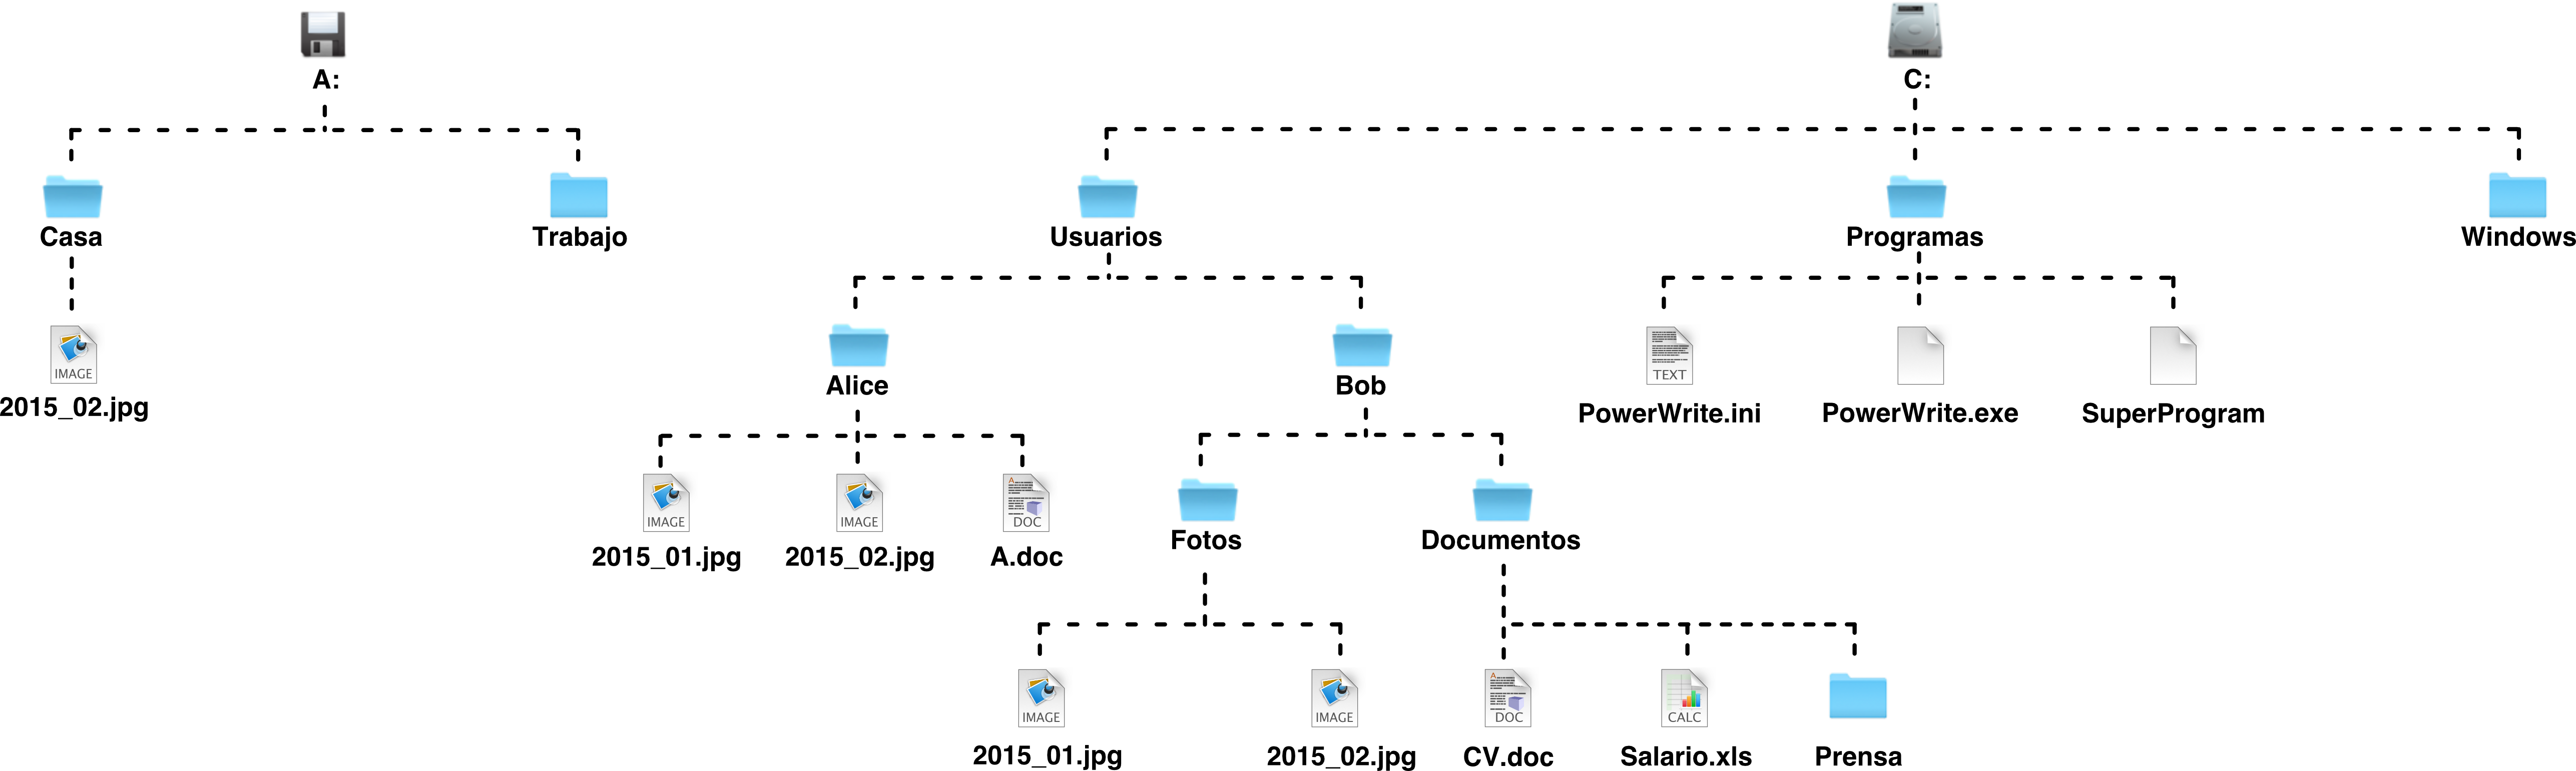
\includegraphics[scale=0.35]{capitulos/informatica/imagenes/directorios_windows_1.png}}

En este sistema hay dos dispositivos de almacenamiento. Un disco extraible ``floppy''
que Windows ha identificado con el nombre ``A:'', y un disco rígido, el cual se
identifica con ``C:''. Es decir, ``A:'', y ``C:'' son las carpetas raíces de cada
uno de los dispositivos de almacenamiento presentes en el sistema.

Dentro del disco rígido hay tres carpetas, ``Usuarios'', ``Programas'' y ``Windows''.
La carpeta ``Windows'' está \textbf{vacía}. Un directorio se denomina vacío
cuando no contiene otras carpetas o archivos en su interior. La carpeta
``Programas'' contiene solamente tres archivos en su interior, ``PowerWrite.ini'',
``PowerWrite.exe'' y ``SuperProgram''. La carpeta ``Usuarios'' tiene dentro
dos carpetas, ``Alice'' y ``Bob'', las cuales a su vez contienen otras carpetas
y archivos en su interior.

Surgen varias cosas de este ejemplo. En primer lugar podemos ver que hay más de
un archivo con el nombre ``2015\_02.jpg''. ¿Significa esto que todos son el mismo
archivo? La respuesta es no, solo son archivos con el mismo nombre, pero el
contenido del mismo podría ser completamente distinto. Podemos así modificar uno
de esos archivos sin afectar el contenido de los otros. También surge la
pregunta ¿Cómo sabe el sistema de cuál de los archivos estamos hablando? La
respuesta es, mediante la ruta absoluta del archivo.

Cuando se trabaja sobre un archivo en el equipo, y aunque transparente para el
usuario en la mayoría de los casos, se debe indicar la ruta completa al archivo,
para que el sistema lo identifique de forma unívoca. Tomemos el ejemplo del archivo
``2015\_02.jpg''; dicho nombre no es único, sino que existen tres archivos con
el mismo en ubicaciones distintas en el equipo. Si deseamos trabajar con cualquiera
de ellos, deberíamos dar al sistema la ruta absoluta de aquel archivo que nos
interesa. Para obtenerla uno debe imaginar una especie de camino que parte desde la
carpeta raíz (por ejemplo, ``C:'') y luego continúa por las lineas punteadas hasta
arribar en el archivo, pasando en el camino por una serie de directorios intermedios
(siempre moviéndose hacia abajo y a los laterales, obteniendo así el camino más corto).
En el gráfico siguiente se muestran tres caminos distintos que llevan a los distintos
archivos con el nombre ``2015\_02.jpg'', marcados cada uno con un color distinto.

\vspace{0.5cm}
\centerline{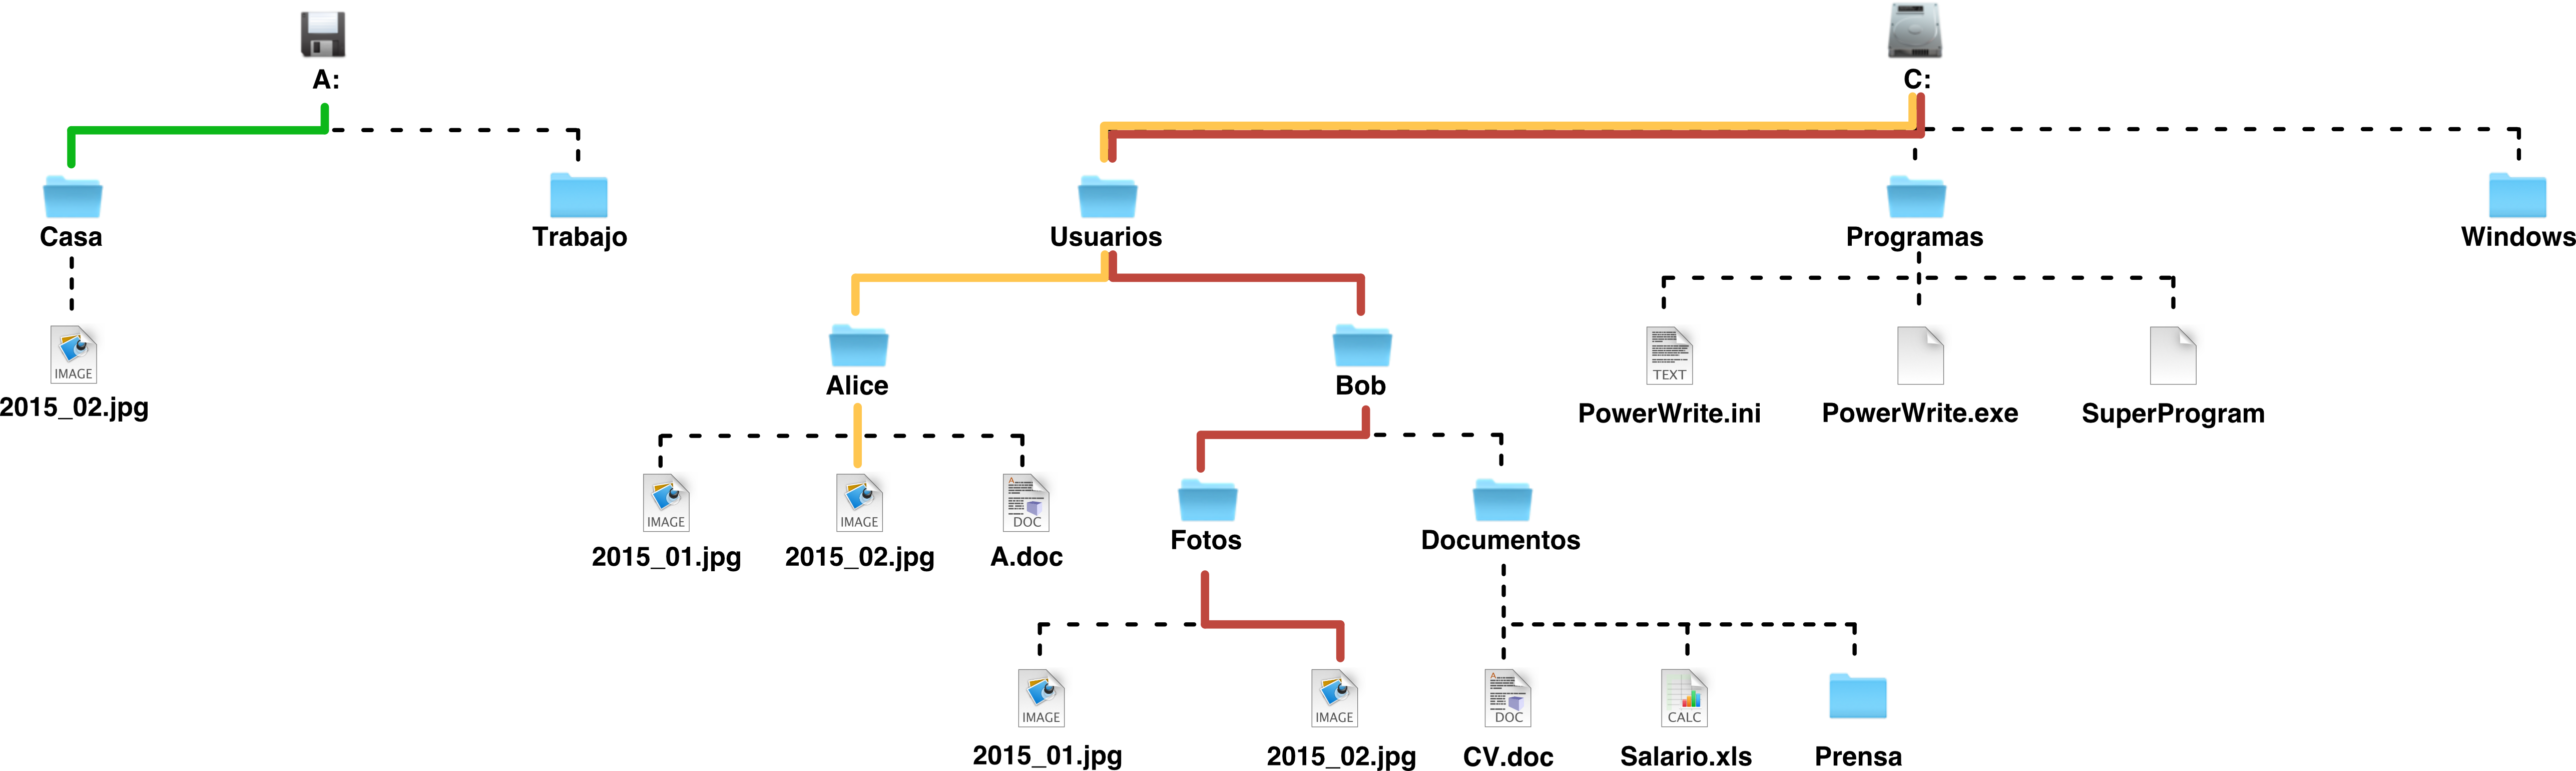
\includegraphics[scale=0.35]{capitulos/informatica/imagenes/directorios_windows_2.png}}

Cada línea corresponde entonces a la ruta absoluta para cada uno de los archivos
con el nombre ``2015\_02.jpg''. La primer línea, la verde, parte desde el disco
floppy ``A:'', pasa por el directorio ``Casa'', para luego arribar en el archivo.
Así, vamos a decir que la ruta a ese archivo es:

\begin{example}
    \textbf{Ruta roja}\\
    A: » Casa » 2015\_02.jpg
\end{example}

En el segundo caso, la ruta amarilla, parte desde el disco rígido ``C:'', y pasa
luego por la carpeta ``Usuarios'', para continuar por ``Alice'' previo a arribar
al archivo. Los pasos serían entonces:

\begin{example}
    \textbf{Ruta amarilla}\\
    C: » Usuarios » Alice » 2015\_02.jpg
\end{example}

Finalmente, la ruta roja parte igualmente desde el disco rígido ``C:'', y pasa
luego por la carpeta ``Usuarios'', pero continua ahora por ``Bob'', luego en
``Fotos'' para arribar ahora si, al archivo:

\begin{example}
    \textbf{Ruta roja}\\
    C: » Usuarios » Bob » Fotos » 2015\_02.jpg
\end{example}

Como vemos, tres archivos con el mismo nombre tienen rutas completamente distintas.
Podemos obtener varias conclusiones de este ejemplo. Por un lado vemos que los
sistemas de archivos con directorios permiten que múltiples archivos se llamen
de la misma forma, ya sea que efectivamente sean el mismo archivo, o que no lo sean.
Por otro lado, no pueden existir nunca dos archivos con el mismo nombre en un
mismo directorio.

Miremos con atención el caso de ``PowerWrite''. Existen dos archivos con ese
nombre en la misma carpeta, sin embargo, tienen distinta extensión. Tenga presente
el lector que siempre que hablamos del nombre de un archivo, en general nos
referimos al nombre y su extensión.

De la experiencia que usted pueda tener con el uso de computadoras, sabrá que
los archivos pueden copiarse, y moverse a diferentes directorios. ¿Qué ocurre
si muevo un archivo de lugar? Lo que sucede es que su ruta absoluta cambia.
Todo esto puede parecer algo menor, pero las rutas absolutas son utilizadas
por los programadores para hacer referencia a archivos que deben estar presentes
en el equipo para que un determinado sistema funcione. Mover un archivo de lugar
puede hacer que todo un sistema falle, pues el archivo no se encuentra en la ruta
que el sistema esperaba. Así también, modificar configuraciones de un sistema que
involucran rutas absolutas sin mover de forma acorde los archivos puede ocasionar
el mismo efecto. Por tanto, entender qué y cómo funcionan las rutas es una parte
fundamental para cualquier persona que quiera comprender un poco más en profundidad
los sistemas informáticos, cualquiera sea su fin.

Es menester mencionar algunos detalles sobre nomenclatura de rutas
en diversos sistemas. Note que en los ejemplos utilizamos el símbolo ``»'' para
separar cada uno de los elementos de una ruta. En realidad cada sistema operativo
puede utilizar una símbolo distinto para separar los elementos de una ruta.
Windows utiliza por convención la barra invertida (\textbackslash). Linux,
macOS, y otros sistemas (aquellos que utilizan la convención de los sistemas
basados en UNIX, y que en general se denominan sistemas basado en UNIX, o sistemas
POSIX) separan los elementos con barra simple (/). Así, las rutas de los ejemplos
de esta sección se escribirían en Windows:
\begin{itemize}
    \item A:\textbackslash Casa\textbackslash 2015\_02.jpg
    \item C:\textbackslash Usuarios\textbackslash Alice\textbackslash 2015\_02.jpg
    \item C:\textbackslash Usuarios\textbackslash Bob\textbackslash Fotos\textbackslash 2015\_02.jpg
\end{itemize}

La convención en sistemas UNIX, es también la utilizada por muchos lenguajes de
programación y de marcado, como veremos más adelante. Utilizando esta convención
las rutas anteriores quedarían.
\begin{itemize}
    \item A:/Casa/2015\_02.jpg
    \item C:/Usuarios/Alice/2015\_02.jpg
    \item C:/Usuarios/Bob/Fotos/2015\_02.jpg
\end{itemize}

Como detalle final, cabe mencionar que los sistemas UNIX no utilizan una letra
para cada uno de los dispositivos, sino que suelen tener un sistema de archivos
que comienza en una carpeta virtual denominada ``/'' (``raíz'' o ``root'').
Los diversos dispositivos son simplemente carpetas dentro de alguna de las
carpetas que tiene ``/'', por ejemplo, la carpeta ``mnt'' o ``mount''. Las rutas
absolutas en dichos sistemas comienzan entonces con la barra simple, para indicar
que parten desde la raíz. Las rutas anteriores podrían verse algo como:
\begin{itemize}
    \item /mount/floppy1/Casa/2015\_02.jpg
    \item /mount/hd0/Usuarios/Alice/2015\_02.jpg
    \item /mount/hd0/Usuarios/Bob/Fotos/2015\_02.jpg
\end{itemize}

Las rutas absolutas son un concepto simple de entender, pero complejo de dominar
sin práctica en su uso. Más difícil aún es el concepto de rutas relativas.

\subsection{Rutas relativas}
\index{Ruta}\index{Ruta Relativa}

Históricamente, los primeros sistemas funcionaban indicándole a la computadora
comandos a realizar, mediante la introducción de las mismas utilizando el teclado.
El usuario solamente visualizaba una pantalla con texto, y el mouse no existía.
En ese contexto, indicar la ruta absoluta de forma constante para cualquier archivo
que el usuario quisiera manipular era sumamente engorroso. Para solucionar esa
molestia surgen dos ideas, la primera es el concepto de \textbf{directorio de
trabajo actual}, y la segunda las \textbf{rutas relativas}.

\begin{definition}
    El \textbf{directorio de trabajo actual} es un directorio de un sistema de
    archivos jerárquico el cual se encuentra asociado de forma dinámica a un
    proceso o tarea del sistema.
\end{definition}

En estos sistemas antiguos, el usuario se encontraba siempre trabajando en un
directorio, el cual era denominado el directorio de trabajo actual. El sistema
operativo mantenía un registro del directorio de trabajo actual, ya que el mismo
podía cambiar a lo largo del tiempo, pudiendo ser modificado por el usuario
mediante la utilización de uno o más comandos. Este concepto viene de la mano
con la idea de \textbf{rutas relativas}.

\begin{definition}
    Una \textbf{ruta relativa} hacia un archivo consiste en la ruta a realizar
    desde un directorio cualquiera para dar con dicho archivo. Si el directorio
    elegido es el directorio raíz del dispositivo en donde se encuentra el archivo,
    la ruta relativa y la ruta absoluta son la misma.\autocite[vid.]{foldoc_relative_2018}
\end{definition}

Una ruta relativa puede indicar donde se encuentra un archivo sin tener que
conocer todas las carpetas del equipo. En particular, en estos primeros sistemas
operativos, uno podía mencionar un archivo con la ruta relativa desde el
directorio de trabajo actual hacia el mismo. Así, sin importar en que carpeta uno
estuviera trabajando, si se deseaba hablar de un archivo en esa carpeta bastaba
solo con el nombre, incluso si la ruta absoluta era larga y compleja.

Veamos un ejemplo en donde el usuario ha decidido que el directorio de trabajo
actual sea la carpeta ``Bob'', dentro de la carpeta ``Usuarios'' en el disco
rígido ``C:''. Es decir, todas las rutas serán relativas a la carpeta
``C: » Usuarios » Bob''.

\vspace{0.5cm}
\centerline{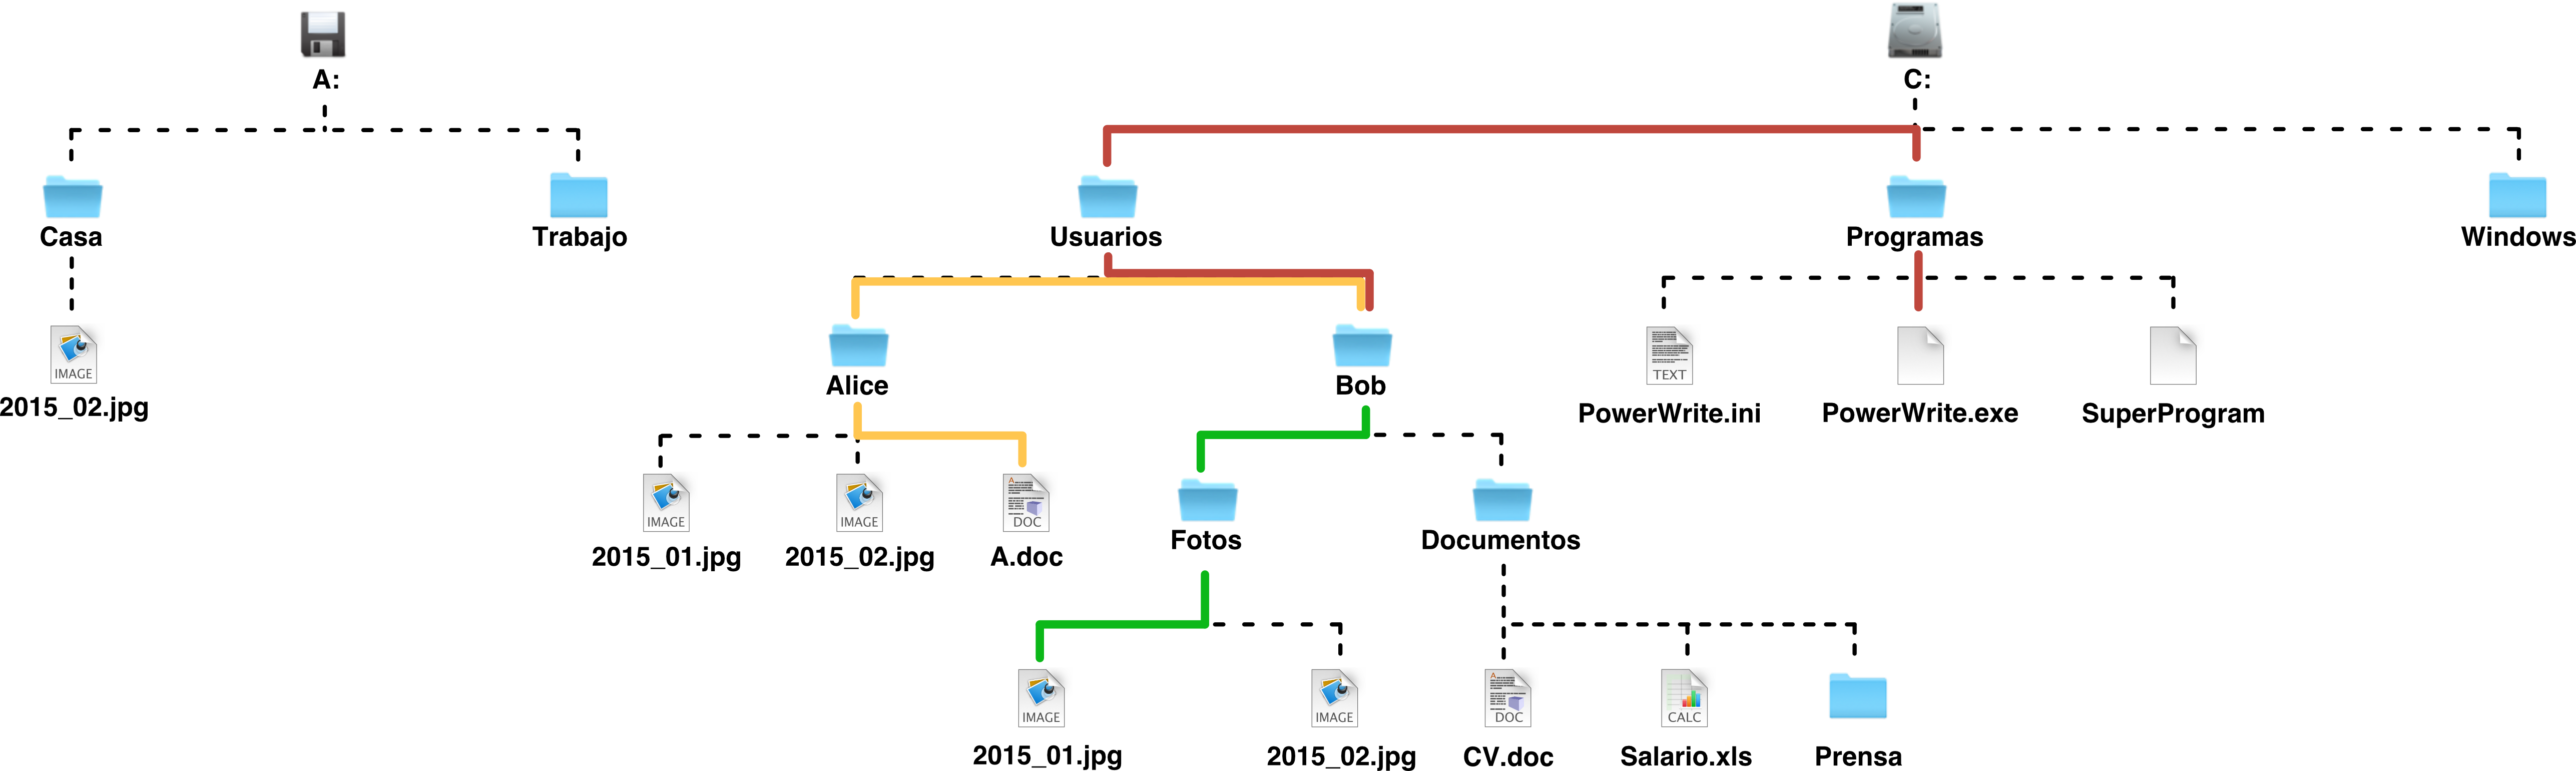
\includegraphics[scale=0.35]{capitulos/informatica/imagenes/directorios_windows_3.png}}

Analicemos primero la ruta verde. Bob quiere acceder al archivo en ``C: » Usuarios
» Bob » Fotos » 2015\_01.jpg''. Como el directorio de trabajo ya es ``C: » Usuarios » Bob'',
basta con poner la ruta desde dicha carpeta (sin incluirla) hasta el archivo.

\begin{example}
    \textbf{Ruta verde}\\
    Fotos » 2015\_01.jpg
\end{example}

Es decir, desde la carpeta ``Bob'' basta ir a la carpeta ``Fotos'' para encontrar
allí el archivo ``2015\_01.jpg''. Note como la ruta siempre va hacia ``abajo'',
es decir, que nos adentramos más en la jerarquía de carpetas, siempre yendo hacia
la carpeta que está dentro de la anterior, y nunca saliendo de la misma.

En el caso de la ruta amarilla esto no es así. Bob quiere acceder al archivo de Alice,
pero dichos archivos no se encuentran dentro de una carpeta en ``Bob'', es decir,
se debe ``subir'' para poder acceder a ellos. Es decir, la ruta relativa debe
dejar constancia de que, en primer lugar, hay que ir de la carpeta ``C: » Usuarios
» Bob'' a ``C: » Usuarios'' en lo que podríamos denominar ``subir un nivel''. La
ruta quedaría algo como:

\begin{example}
    \textbf{Ruta amarilla}\\
    \textasciicircum ~ » Alice » A.doc
\end{example}

Es decir, partiendo de la carpeta ``Bob'', vaya a la carpeta inmediatamente
arriba (llamada \textbf{padre}). Luego, desde ahí, vaya a la carpeta ``Alice'',
una vez allí encontrará el archivo ``A.doc''.

En el caso de la ruta roja el proceso es el mismo, aunque en este caso no basta
con subir un nivel, sino que tenemos que subir varias veces.

\begin{example}
    \textbf{Ruta roja}\\
    \textasciicircum ~ » \textasciicircum ~ » Programas » PowerWrite.exe
\end{example}

En este caso la ruta absoluta hubiera sido más corta y sencilla que la ruta relativa,
sin embargo es interesante ver como una ruta relativa puede aplicar en cualquier
punto de la jerarquía de carpetas, e independientemente de la carpeta.

Nuevamente el símbolo ``\textasciicircum'' que utilizamos para indicar ``ir un nivel hacia arriba''
se representa distinto en distintos sistemas. Sin embargo, los sistemas más populares
usan todos la misma convención: ``..''. Las rutas anteriores quedarían en Windows:

\begin{itemize}
    \item Fotos\textbackslash 2015\_01.jpg
    \item ..\textbackslash Alice\textbackslash A.doc
    \item ..\textbackslash ..\textbackslash Programas\textbackslash PowerWriter.exe
\end{itemize}

Y en los sistemas UNIX
\begin{itemize}
    \item Fotos/2015\_01.jpg
    \item ../Alice/A.doc
    \item ../../Programas/PowerWriter.exe
\end{itemize}

Una propiedad interesante de las rutas relativas es que, dado un directorio
como directorio de trabajo actual, todas las rutas relativas desde el mismo
hacia archivos o carpetas que este contenga son iguales independientemente de
donde esté ubicado el directorio en el equipo. Esto resulta muy útil a las personas
de sistemas, pues un archivo de configuración o programa que utilice esta técnica
para hacer mención de sus archivos puede ser copiado o movido a otro lado sin
perjudicar su funcionamiento, dado que no se copie solo el archivo, sino todos
los archivos que están en la carpeta del programa. Veremos más este detalle en
secciones futuras.

\subsection{Universal Resource Identifier}
\index{URI}\index{URL}

Imaginemos ahora una serie de computadoras conectadas entre si. Es decir, una red
de computadoras. Las redes permiten compartir recursos, los cuales, entre otras
cosas, incluyen archivos y directorios. Por tanto, es importante poder identificar
de forma única un archivo, ya no en un equipo, sino en toda una serie de equipos.
Si la cantidad de máquinas es grande, nombrar con una única letra cada dispositivo
de la red se vuelve imposible. Para solucionar este problema surgen el \textbf{
identificador universal de recursos}, o en inglés \textbf{universal resource
identifier (URI)}. Pero antes de entender que son los URIs, veamos un momento
como se identifica un equipo en una red.

Cuando se cuenta con diversas computadoras conectadas a una red, se debe poder
hacer mención a una máquina en particular, diferenciándola del resto de las de
la red. Así, los sistemas de software de red (por ejemplo, aquellos incluidos
en un sistema operativo o incluidos en dispositivos como routers) asignan a cada
equipo un número único, conocido como \textbf{dirección IP}. 

Otra técnica para hablar de un equipo único en una red consiste en asignarle un
\textbf{nombre de dominio}. Los nombres de dominio son identificadores en texto,
en lugar de numéricos, por lo que son más fáciles de recordar por los seres humanos.
Un sistema especializado mantiene registro de los nombres asignados para que no
existan dos equipos con el mismo nombre, además de recordar la asociación entre
el nombre de dominio y la dirección IP a la que corresponde.

Tal vez haya visto en algún momento estas formas de identificar computadoras
al navegar por Internet, pues Internet no es más que una gran red donde el
usuario simplemente solicita archivo a diversos equipos. Una dirección IP
se compone en realidad de 4 números entre 0 y 255 cada uno, los cuales se
escriben separados por puntos (ej. ``125.65.92.135''). En cambio los nombres
de dominio suelen consistir en dos partes, de las cuales la primera suele ser
un nombre que identifica a una empresa u organización, y la segunda, que consiste
en un conjunto de 2 y/o 3 letras que identifican el tipo de organización (empresa,
ONG, entidad educativa, etc.) y/o el país al que pertenece (ej. ``google.com.ar'',
``wikipedia.org'').

Ahora bien, una URI se compone entonces de diversas partes. En primer lugar un
protocolo, que le indica a los equipos de que forma se espera que se transfiera
el archivo de una máquina a la otra, seguido por alguna forma de identificador
de equipo (ya sea la dirección IP o un nombre de dominio) y luego una ruta hacia
el archivo en cuestión. Como por motivos de seguridad las computadoras no
comparten en la red todos los archivos sino una carpeta específica del equipo,
la ruta de la URI no es una ruta absoluta, sino relativa a la carpeta compartida.
\autocite{rfc7320_2014}

\vspace{0.5cm}
\centerline{
\includegraphics[]{capitulos/informatica/imagenes/uris.png}}

Un URI también puede ser llamado URL (Universal Resource Locator). Si bien hay
pequeñas diferencias técnicas entre uno y otro concepto, los términos hoy en día
se suelen utilizar de forma prácticamente intercambiable. Además, tanto los URI
como los URL pueden contener otros elementos, como sub-dominios, puerto, queries,
y fragmentos, que no analizaremos aquí.

\begin{definition}\index{URI}\index{Identificador de Recursos Universal}
    Un \textbf{identificador de recursos universal} es una cadena de texto
    capaz de identificar un recurso en un equipo específico dentro de una
    red de computadoras.
\end{definition}

El concepto de URI no es nada más que el mismo concepto de ruta expandido hacia
las redes, de forma tal que cualquier archivo (que sea accesible) tenga una forma
única de identificarse.

Cabe destacar como detalle adicional que el símbolo utilizado en una URI para
separar los elementos de la ruta sigue el estándar de los sistemas UNIX, es decir,
con barra símple (/). Esto quiere decir que, cuando se accede a un archivo en un
sistema Windows desde Internet, las barras invertidas de la ruta al archivo en
Windows deberán ser reemplazadas con barras simples.

\subsection{Programas, Editores y Visualizadores}
\index{Programa}

Los programas son uno de los elementos de software que más utilizamos. Son lo que
provee a nuestra computadora de diferentes funcionalidades especificar, y nos
permite realizar tareas sumamente diversas con un mismo equipo.

A diferencia del resto de los archivos del equipo, un programa es un
archivo ejecutable. Es decir, al pedirle al sistema operativo que abra el
archivo de un programa, lo que este hará será ejecutarlo.

Ejecutar un programa consiste simplemente en llevar adelante una serie de pasos
que el programa define. Estos pasos pueden ser muchos, y muy diversos, dando lugar
a programas completamente distintos. Además, pueden incluir elementos visuales, como
botones, imágenes y otros, para simplificar el uso para el usuario final.

\wraprimage[0.5]{capitulos/informatica/imagenes/word.png}
{Banner publicitario de Microsoft Word con su aplicación para PC y teléfonos móviles.}
{Imagen de Microsoft.}

Los programas pueden agruparse en categorías según diversos criterios. Por ejemplo,
podríamos decir que hay programas que son ``accesorios'', elementos prácticos que
el usuario puede requerir y conviene tener a manos, como una calculadora o un anotador.
También hay programas que podrían entrar en una categoría ``reproductores de video'',
que permiten al usuario ver videos en uno o más formatos, así como controlar
factores como el sonido y otros.

Una categorización interesante que nos interesa mencionar aquí tiene que ver con
como tratan los programas a los archivos que manipulan. En particular, podemos
determinar dos grandes categorías, \textbf{visualizadores} y \textbf{editores}.

Un visualizador permite simplemente ver los datos que se encuentran almacenados
en un archivo, pero no modificarlos. Por ejemplo, un reproductor de video permite
ver una película digital, pero no modificarla. Un navegador de internet permite
ver páginas web, pero nuevamente, no pueden modificarse usando ese programa.

\begin{definition}\index{Visualizador}
    Un \textbf{visualizador} es un programa que permite ver el contenido de
    archivos que tienen algún formato específico.
\end{definition}

Los editores en cambio permiten manipular la información del archivo, alterando
sus contenidos. Por ejemplo, un editor de sonido, o un manipulador de imágenes
permiten editar audio o fotografías digitales, y no son los programas que el
usuario utilizaría si lo que le interesa es escuchar música o ver fotografías.

\begin{definition}\index{Editor}
    Un \textbf{editor} es un programa que permite crear y modificar el contenido
    de archivos que tienen algún formato específico.
\end{definition}

Existen programas que cumplen ambas funciones al mismo tiempo. Por ejemplo
Microsoft Word es el programa que se usa tanto para editar archivos de documentos,
como para visualizar su contenido. Los documentos de Word no pueden (en principio)
verse con otros programas que no sean Word, y tampoco editarse con otros programas.

\index{Editor de Texto}
Una mención especial merecen los \textbf{editores de texto}. Un editor de texto
permite editar el contenido de un archivo de texto sin formato. Como veremos más
adelante, algunos formatos de archivo no codifican la información en binario,
sino como texto. Para estos archivos, un editor de texto permite modificar su
contenido, independientemente si codifican imágenes, documentos, u otros.

\section{Programas y Lenguajes}

Un programa es el resultado del trabajo de un desarrollador de software (dentro
de otros elementos), por lo que para realizar un programa se requiere de una serie
de conocimientos técnicos específicos que permiten desarrollarlo.

Resulta interesante tener una noción básica de la forma en la que se realiza 
desarrolla un programa (sin internalizar en los conceptos específicos). Para
encarar esta tarea es prioritario comprender el concepto de lenguaje, desde un
punto de vista técnico.

\subsection{Lenguajes}
\index{Lenguaje}

El lenguaje nos posibilita comunicarnos con quienes nos rodean, pero también
con otras personas a lo largo del tiempo y el espacio. Gracias al lenguaje
es que hoy tenemos registro de lo que pasó en tiempos distantes, en lugares remotos.

\begin{definition}
    Un \textbf{lenguaje} es un sistema de comunicación, el cual se encuentra definido y
    estructurado, y que posee un contexto de uso (es decir, se puede establecer
    una semántica a determinados elementos).
\end{definition}

\wraplimage{capitulos/informatica/imagenes/banderas.jpg}
{Banderas de diversos paises ondeando en la plaza de los Juegos Panamericanos en Rio de Janeiro.}
{Imagen de Wilson Dias / Ag\^encia Brasil}

Puede sonar complejo en la definición, pero utilizamos el lenguaje todo el tiempo.
La forma más común de lenguajes son los idiomas, como el español o el inglés.
Cada uno de los idiomas define un conjunto de símbolos que son válidos, por ejemplo,
el español cuenta con la letra ``Ñ'', que no está presente en el inglés. Cualquier
palabra que use dicho símbolo es inválida en inglés, y por tanto no forma parte de
ese lenguaje, mientras que en cambio, si puede formar parte del nuestro. También
las reglas de un idioma (que son extremadamente complejas) determinan que textos
son válidos y cuales no. En primer lugar, la regla más sencilla determina palabras
que existen en el lenguaje (dadas muchas veces por los diccionarios oficiales).
La gramática determina luego como unir esas palabras para que cobren sentido.

No solo hay idiomas que han surgido y evolucionado naturalmente, sino que pueden
existir lenguajes creados de forma artificial con fines específicos. Por ejemplo,
algunas series de televisión han creado lenguajes con fines artísticos, como la
serie de ciencia ficción Star Trek y el lenguaje Klingon, o Game of Thrones (
basada en los libros de George R. R. Martin) y el Idioma Dothraki.\autocite{littaur_2017}

Pero también han habido intentos más nobles, como el Esperanto. Creado por 
L. L. Zamenhof, un oftalmólogo polaco, el Esperanto surge con la idea de que se
transforme en un idioma capaz de ser fácilmente aprendido y hablado por cualquier
persona en el mundo. La intención última era unir a la humanidad bajo un mismo
lenguaje universal (como segunda lengua, sin reemplazar los idiomas oficiales
que ya tenían las distintas naciones). El Esperanto es la
lengua planificada más expandida y utilizada en el mundo hoy en día, y es
reconocida por instituciones como la UNESCO.

\index{Sintaxis}\index{Semántica}
Todo lenguaje está compuesto de dos partes, una \textbf{sintaxis} y una
\textbf{semántica}. La sintaxis determina los símbolos y las reglas que es posible
utilizar en el lenguaje, mientras que la semántica determina que significado le
asociamos a una determinada sintaxis. Por ejemplo, las expresiones ``Me baño en
el río'' y ``Me río en el baño'' son muy similares en cuanto a sintaxis se refiere,
pero la semántica asociada, es decir, el significado de esas dos frases, es completamente
distinto.

Pensemos también en una frase como ``lo voy a tomar''. ¿Cuál es la semántica de
dicha frase?. A priori es difícil saberlo pues la palabra ``tomar'' tiene
muchos significados distintos dependiendo del contexto. Puede que se esté hablando
de un cuarto de un hotel, o de un transporte público. También podría ser que la
frase se refiera a una bebida, o a un helado. Incluso la palabra tomar puede
referirse a agarrar un objeto. Decimos entonces que la frase es \textbf{ambigua},
pues su significado no queda claro si no se cuenta con el contexto subyacente.

La ambigüedad es una problemática que a los humanos no nos molesta demasiado,
pues somos capaces de analizar contextos y desambiguar rápidamente una frase
basándonos en la información que tenemos. Las máquinas por otro lado, no tienen
esa capacidad. Por tanto, es difícil (imposible prácticamente) comunicarse con
una computadora utilizando los idiomas que hablamos a diario. Por eso surgen
lenguajes especialmente diseñados para tal fin, y que tienen como principal
característica el no presentar ambigüedades. Estos lenguajes se conocen como
\textbf{lenguajes formales}.

\begin{definition}\index{Lenguaje Formal}
    Un \textbf{lenguaje formal} es un lenguaje cuyos símbolos y
    reglas para unir esos símbolos están formalmente especificados.
    Al conjunto de los símbolos primitivos se lo llama \textbf{alfabeto}, y
    al conjunto de las reglas se lo llama \textbf{gramática formal}.\autocite{sunitha_2015}
\end{definition}

Dentro de los lenguajes formales podemos identificar dos grandes categorías:
los \textbf{lenguajes de programación}, cuya finalidad es poder escribir programas de
computadora, y los \textbf{lenguajes de marcado}, cuyo fin es describir datos que un 
programa puede luego interpretar.

\subsection{Lenguajes de programación}
\index{Lenguaje de Programacion@Lenguaje de Programación}

Los \textbf{lenguajes de programación} consisten en un conjunto de comandos (llamadas
a veces instrucciones) que la computadora es capaz de entender. Mediante una
secuencia de estas instrucciones se pueden lograr complejos programas que
realizan diversas tareas. Así, puede procesar datos que provienen de sensores,
o que son ingresados por el usuario, pueden imprimir información en pantalla,
o transmitir información por la red, dependiendo de qué es lo que el programador
haya determinado.

Cabe destacar que, en general, los comandos incluidos en un lenguaje suelen
realizar tareas sencillas y bien puntuales. Por ejemplo, es casi seguro que un
lenguaje de programación no va a incluir un comando para calcular la hipotenusa
de un triangulo sabiendo los catetos del mismo. Sin embargo, una persona con
conocimientos del teorema de Pitágoras puede llegar al mismo resultado utilizando
una serie de comandos más simples (multiplicación, radicación y sumas). A
continuación hay un ejemplo de programa que calcula la hipotenusa de un triangulo
dados sus catetos.

\begin{example}
    \textbf{código de ejemplo para el cálculo de hipotenusa de un triangulo}

    \begin{enumerate}
        \item Leer del teclado el número que el usuario ingresa como C1
        \item Leer del teclado el número que el usuario ingresa como C2
        \item CSQ1 $\leftarrow$ C1 * C1
        \item CSQ2 $\leftarrow$ C2 * C2
        \item HSQ $\leftarrow$ CSQ1 + CSQ2
        \item H $\leftarrow$ raíz de HSQ
        \item Informar al usuario en pantalla el valor H
    \end{enumerate}
\end{example}

\begin{definition}
    Un \textbf{lenguaje de programación} es un lenguaje formal que especifica
    una serie de instrucciones para que una computadora procese y produzca diversas
    clases de datos. Los lenguajes de programación se usan para crear programas
    de computadora.\autocite{sebesta_2005}
\end{definition}

\wraprimage[0.5]{capitulos/informatica/imagenes/tiobe_programming_languages.png}
{Gráfico de burbuja que muestra la popularidad de diferentes lenguajes de programación
según el Indice TIOBE.}
{Imagen de Untapt con datos de TIOBE.}

En este código ``*'' se utiliza como símbolo para multiplicar, y ``$\leftarrow$''
indica que el resultado de la cuenta debe ser recordado con un nombre (que
figura a la izquierda de la flecha) para poder ser utilizado posteriormente.

No existe un único lenguaje de programación, sino que hay cientos de ellos, cada
uno con sus propias características, y diseñados para satisfacer necesidades
específicas. Así, \textbf{no existe un ``mejor lenguaje''}, sino que existen lenguaje
más o menos apropiados para solucionar un determinado problema. Por otro lado, muchos
lenguajes distintos permiten solucionar los mismos problemas, pero con diferentes
enfoques, por lo que el \textbf{programador puede elegir aquel que más se adapte a su
necesidad, pero también a sus preferencias personales}.

\index{Compilador}\index{Compilar}
Pero, si las computadoras trabajaban con binario, ¿Cómo hacen para entender ese
programa?. La respuesta radica en utilizar un programa. El programador genera un
archivo con texto, similar al expuesto arriba, y lo guarda en el equipo. Luego,
le indica a un programa especial, llamado \textbf{compilador}, que procese ese
archivo para transformar el texto que contiene en una secuencia de unos y ceros
que correspondan a un programa que realiza las tareas descriptas en el archivo.
Al proceso mencionado, que realiza el compilador, se lo conoce como \textbf{compilar}.

\textbf{El compilador transforma entonces una secuencia de unos y ceros que representan
texto, en una secuencia de unos y ceros que representan un programa}

\index{Codigo Fuente@Código Fuente}\index{Codigo Objeto@Código Objeto}
El archivo que contiene el texto que describe el programa se conoce como
\textbf{código fuente} del programa, mientras que el programa resultante se conoce como
\textbf{código objeto} o \textbf{código compilado}.

\begin{definition}\index{Compilador}
    Un \textbf{compilador} es un programa que transforma un archivo con código fuente
    en un archivo con código objeto, capaz de ser ejecutado en una computadora.
\end{definition}

\index{Interprete}\index{Interpretar}
También existen algunos lenguajes que no trabajan de esta forma, sino que un programa
va leyendo cada una de las líneas del programa, y lleva adelante la acción descripta
para esa línea previo a leer la siguiente linea. Esto se conoce como \textbf{interpretación},
y el programa que realiza esa tarea se conoce como \textbf{interprete}.

\begin{definition}\index{Interprete}
    Un \textbf{interprete} es un programa que ejecuta paso a paso cada uno de los
    comandos descriptos en un archivo con código fuente.
\end{definition}

\begin{knowwhat}[Simplificación]
    La realidad es que el funcionamiento de los compiladores e interpretes es
    bastante más compleja. Hoy en día muchos interpretes realizan pasos de
    pre-compilación, y muchos compiladores funcionan con técnicas JIT. También
    se está obviando el tema de máquinas virtuales, lo cual representa un
    componente muy importante en los procesos de ejecución de programas actuales.

    Estos temas merecen un trabajo mucho más en profundidad, así como un bagaje
    de conocimientos mucho mayor al que el presente intenta proporcionar.
\end{knowwhat}

Es importante a tener en cuenta que, ni los compiladores ni los interpretes trabajarán
con cualquier texto, sino que esperan texto escrito en un lenguaje específico.
Es decir, el compilador del lenguaje C, no funcionará si se intenta procesar con
el un archivo con código Python. Así, cada lenguaje tiene su propio compilador,
o su propio interprete (o ambos).

\index{Lenguaje Compilado}\index{Lenguaje Interpretado}
El lector puede o podría encontrar en diversa bibliografía términos como
``\textbf{lenguajes compilados}'' o ``\textbf{lenguajes interpretados}''. Esta
categorización responde simplemente al hecho de que, en general, el autor del
lenguaje provee asociado a la definición su lenguaje (gramática, semántica, etc.),
la herramienta que permite generar programas en dicho lenguaje (la cuál suele ser
o bien un compilador, o bien un interprete). Sin embargo, nada evita que
un lenguaje que era inicialmente distribuido con un interprete pueda ser luego
distribuido con un compilador, sin alterar el lenguaje en si. Esto quiere
decir que la categorización anterior es incorrecta, pues ser compilado o
interpretado no es una característica del lenguaje, sino de la herramienta que
lo acompaña.

\index{Lenguaje de Bajo Nivel}\index{Lenguaje de Medio Nivel}\index{Lenguaje de Alto Nivel}
Otra categorización que suele realizarse es la que diferencia lenguajes entre
aquellos que son de \textbf{bajo nivel} y los que son de \textbf{alto nivel},
distinguiendo incluso en ocaciones con un \textbf{medio nivel}. Los lenguajes
de bajo nivel suelen proveer comandos que están asociados a las operaciones que
puede realizar el hardware del equipo. Así, para cada comando, seguramente haya
un circuito específico dentro del equipo. En cambio los lenguajes de alto nivel
proveen construcciones más complejas, que no necesariamente se traducen a circuitos,
y que están más ligadas a ideas o conceptos que el desarrollador puede querer
expresar. Cuando el desarrollador realiza el programa, primero piensa la idea,
la cual está expresada en lenguaje natural. Sin embargo, luego debe plasmar esa
idea en el lenguaje de programación específico. Cuanto más parecido sea el lenguaje
de programación a las ideas mentales del programador, más fácil será ese proceso.
\autocite{wexelblat_1981}

\index{Paradigma}\index{Paradigma Imperativo}\index{Paradigma Orientado a Objetos}
\index{Paradigma Funcional}
Una última categorización tiene que ver con la forma en la que el lenguaje
permite estructurar ideas. Esto se conoce como el \textbf{paradigma} del lenguaje.
Los primeros lenguajes de programación masivos utilizaban el \textbf{paradigma
imperativo}, que consiste en secuencias de instrucciones dadas al equipo una tras
otra. Existen otros paradigmas, como el \textbf{paradigma funcional}, más ligado
a los desarrollos de teoría de la computación formal desarrollados por Alonzo
Church, o la \textbf{programación orientada a objetos}, que utiliza procesos
de abstracción conocidos como objetos para modelar los datos, y la comunicación
entre ellos para modelar las transformaciones de esos datos. También existen
otros paradigmas, más específicos y menos difundidos, y lenguajes que permiten
escribir programas usando más de un paradigma al mismo tiempo.


\subsection{Lenguajes de marcado}

\wraprimage[0.5]{capitulos/informatica/imagenes/whatsapp.png}
{Whatsapp trae incluido un lenguaje de marcas, que permite utilizar símbolos
de texto simple al momento en el que el emisor redacta el mensaje para que el
receptor visualice porciones del texto recibido con un formato particular.}
{Imagen propia.}

\index{Lenguaje de Marcado}
Otro tipo de lenguajes formales son los \textbf{lenguajes de marcado}. Estos
lenguajes tienen como función describir datos, donde ``datos'' puede ser cualquier
cosa. Por ejemplo, existen lenguajes de marcado que describen publicaciones en foros,
otros que describen páginas de wikis (como Wikipedia), otros que describen
documentos, otros para imágenes, otros para páginas web, etc.

Recordemos que todas estas cosas podrían ser fácilmente representadas mediante
archivos con diferente formato, esto es, con una codificación distinta del
binario que representa el dato en el archivo. En los lenguajes de marcado,
no se requieren diferentes formatos de archivo, sino que siempre se trabaja
con texto plano, por lo que los datos \textbf{pueden ser editados con un editor
de textos}.

La gracia es que el \textbf{texto contiene una serie de símbolos especiales, llamadas
marcas} (de ahí el nombre de ``lenguajes de marcado''). Estas marcas representan
diferentes elementos semánticos dentro del documento, indicando por ejemplo, que
una determinada parte se debe ver en negrita o en itálica, o que un determinado
texto debería ser considerado un título, o que se debería insertar una tabla de
datos en determinado lugar, o simplemente dando información semántica sobre
la parte ``marcada''. Estas marcas pueden luego ser interpretadas luego por un
visualizador, que las mostrará como elementos visuales, o ser utilizadas por
un programa para realizar tareas especificas de acuerdo a las mismas.

Existen cientos de lenguajes de marcado, cada uno intentado resolver una problemática
distinta. Cada lenguaje define entonces que símbolos representan marcas, y como
deben ser utilizados en el texto, así como la asociación semántica de cada
marca.\autocite{coombs_1987}

\begin{definition}\index{Lenguaje de Marcado}
    Un \textbf{lenguaje de marcado} consiste en una codificación que incorpora
    en un archivo de texto plano que junto con el texto incorpora una serie de
    marcas o etiquetas que contienen información sobre la semántica, la
    estructura o la forma de presentar el texto.
\end{definition}

\begin{knowwhat}
    Un archivo de texto solo contiene información del texto que contiene, es decir
    de las letras que están escritas. No maneja ninguna otra información, como
    si las letras están en negrita, itálica o de algún color en particular.
    Sin embargo, muchos editores de texto diseñados para programar ofrecen una
    característica conocida como ``syntax highlighting'' o ``code styling'', que
    colorea partes específicas del código, lo que le permite al desarrollador
    tener un panorama visual más ameno, facilitando su tarea.

    Este libro utiliza coloreo en los lugares en donde se muestra
    código para hacer más fácil la comprensión del mismo.
\end{knowwhat}

Analicemos un ejemplo sencillo. El lenguaje de marcado de los \textbf{archivos
de inicialización de Windows}, o archivos \textbf{.ini} consiste en texto que
debe estructurarse en una serie de líneas. Cada línea consiste en un par de
elementos, donde el primero, el de la izquierda, es conocido como ``clave'',
y el segundo como ``valor''. Ambos elementos se encuentran separados con un
signo ``='' entre ambos. Adicionalmente, un conjunto de líneas con pares clave
valor pueden estar antecedidas con un nombre, colocado entre corchetes en la
línea inmediatamente superior al conjunto, de forma tal de agruparlas bajo
un mismo identificador. Finalmente, cualquier línea que comience con el símbolo 
``';'' (punto y coma) corresponde a un comentario, y el texto de dicha línea no
representa datos relevantes para el archivo, sino información para el desarrollador.
\autocite{getPrivateProfileString_2018}

Todas estas reglas pueden parecer complejas de entender, pero en realidad es uno
de los lenguajes de marcado más sencillos que existe, aunque algunos autores
consideran que es un lenguaje de configuración, más que de marcado.

Pero ¿Para qué sirve un archivo de inicialización de Windows? Bien, tanto
el sistema operativo como diversas aplicaciones pueden utilizar el archivo
para establecer preferencias del usuario. Por ejemplo, el código
ficticio que se presenta a continuación podría utilizarse para configurar un
navegador web:

\begin{example}

    \textbf{contenido hipotético de un archivo .INI}

    \begin{lstlisting}[language=ini]
[Red]
; Poner UsarProxy=1 si no hay cortafuegos
UsarProxy=1
Proxy=192.168.0.1

[Preferencias]
PaginaInicio=https://unq.edu.ar
Maximizar=1
    \end{lstlisting}
\end{example}

Las marcas en un archivo INI consisten en el símbolo ``;'', que marca comentarios,
o los caracteres ``\lbrack'' y ``\rbrack'' que determinan el nombre de un grupo,
así como el signo ``='' que separa la clave del valor en cada línea. El salto
de línea, aunque no es un símbolo visible, también es considerado una marca,
porque brinda información (termina un par clave valor y comienza otro).

Los archivos de configuración de Windows son un formato de archivo sencillo,
pero hoy en día ya obsoleto.

\index{XML}
Otros lenguajes de marcado incluyen \textbf{JSON} o \textbf{XML}, los cuales
son utilizados para intercambios de datos en la web o configuración de aplicaciones
más modernas. A continuación se deja un ejemplo sencillo de \textbf{XML}:\autocite{marshal_2000}

\begin{example}
    
    \textbf{Una receta de cocina codificada en un archivo XML}


    \begin{lstlisting}[language=XHTML]
<Receta>
    <Nombre> Banana con Dulce de Leche </Nombre>
    <Descripción> El mejor postre </Descripción>
    <Ingredientes>
        <Ingrediente> Banana </Ingrediente>
        <Ingrediente> Dulce de Leche </Ingrediente>
    </Ingredientes>
    <Utensilios>
        <Utensilio> Cuchara </Utensilio>
    </Utensilios>
    <Pasos>
        <Paso>Pelar la banana</Paso>
        <Paso>Destapar el frasco de dulce de leche</Paso>
        <Paso>Colocar la cuchara en el frasco</Paso>
        <Paso>Tomar una gran cucharada de dulce de leche</Paso>
        <Paso>Untar el dulce de leche en la banana</Paso>
        <Paso>Comer la banana</Paso>
        <Paso>Repetir el proceso si fuera necesario</Paso>
        <Paso>Cerrar frasco y lavar cuchara</Paso>
    </Pasos>
</Receta>
    \end{lstlisting}

\end{example}

El archivo anterior describe una receta de cocina de un típico postre argentino.
El lenguaje XML contiene como marcas un elemento conocido como \textbf{etiqueta}.
La etiqueta consiste en un nombre colocado entre los caracteres ``<'' y ``>'',
si es de apertura, o ``</' y ``>'' si es de cierre. Cada etiqueta puede contener,
o bien texto, o bien otras etiquetas.

XML permite definir los nombres de las etiquetas, y estructurarlas como se desee.
Por eso, este lenguaje es ampliamente utilizado para describir información.
XML es sumamente flexible, y es considerado el padre de decenas de lenguajes de
marcado. Por ejemplo, se utiliza para definir documentos y planillas de cálculo
en los formatos de documento libre ODT y ODS (archivos similares a los de Word y
Excel), como así también para describir imágenes en el formato SVG. La diferencia
de estos lenguajes de marcado particulares con XML radica en que no cualquier
etiqueta es válida, y no pueden tampoco anidarse de cualquier forma, sino que
deben cumplir una serie de restricciones adicionales.

\index{HTML}
Dentro de los lenguajes que descienden de XML se encuentra \textbf{HTML}, o
\textbf{HyperText Markup Language}, en español ``lenguaje de marcado de hipertexto''.
Este es tal vez el lenguaje de marcado más popular y más vastamente utilizado de
la historia. Esto se debe a que HTML es el lenguaje con el que se \textbf{describen
las páginas web}. Los elementos de una página web son estandarizados, y están
dados por las etiquetas que el lenguaje define. Por ejemplo, la etiqueta
``<a>'' define un enlace a otro sitio web, o la etiqueta ``<img>'' permite insertar
una imagen.

Luego, un programa especializado, conocido como \textbf{browser} o \textbf{navegador
web}, actúa como visualizador de estos archivos, mostrando los elementos visuales
que el autor haya escrito, sin mostrar las etiquetas.

La combinación de las distintas etiquetas, estructuradas de diversas formas,
puede dar lugar a las más diversas y creativas páginas web que uno pueda desear.
HTML se combina con otros lenguajes, como CSS, y JavaScript, para lograr sitios
web interactivos y con grandes características visuales. Ejemplos y detalles de
este lenguaje se pueden ver en el anexo \ref{HTML}.

\begin{knowwhat}\index{Browsers}
    Casi todos los \textbf{browsers} permiten ver el \textbf{código fuente} de
    la página web que el usuario está navegando. No solo eso, sino que algunos
    incluyen herramientas que sirven a los desarrolladores para analizar, escribir,
    y reparar las páginas que escriben, permitiendo incluso modificar el código
    de páginas remotas de forma local y temporal.
\end{knowwhat}

\textbf{Markdown} es otro interesante lenguaje de marcado. Es ideal para escribir
pequeños documentos informativos, como puede ser documentación, o correos
electrónicos. La ventaja fundamental de Markdown radica en que no se requiere de
un visualizador especializado para comprender el documento, sino que el mismo
código fuente permite visualizar el contenido de forma clara. Un pequeño resumen
del lenguaje se puede ver en el anexo \ref{Markdown}.

\section{Modelos de comercialización de software}

\subsection{Copyright}

\index{Copyright}\index{Derecho de autor}
Debe comprenderse que el software hoy en día goza de \textbf{derechos
de autor} o \textbf{copyright}. Es decir que el autor de un programa goza de todos
los derechos legales de explotación del mismo. Es decir, el autor puede determinar
cosas como la forma en la que el software se vende, alquila o licencia, o cosas
como para que fines puede ser utilizado su programa, si puede ser utilizado como
parte de otros programas, si puede ser utilizado comercialmente, etc.

\begin{definition}
    El \textbf{derecho de autor} (o \textbf{copyright}, por su voz inglesa) consiste
    en un conjunto de normas jurídicas que defienden el derecho moral de los autores
    de obras literarias, artísticas, musicales, científicas, didácticas y de software,
    ya sea publicada o inédita, para explotar dicha obra comercialmente en cualquier
    forma que considere por un periodo de tiempo determinado.\autocite{oxford_copyright_2018}
\end{definition}

El modelo actual de comercialización de software nace en la época de 1970, con la
aparición de las primeras microcomputadoras. Los fabricantes de estas primeras
computadoras instalaban  software de fabrica para venderlo como un valor
agregado a sus equipos. Sin embargo, estos programas solo funcionaban en la
máquina del fabricante, y por tanto uno quedaba atado a este para mantener
compatibilidad de los productos. Además esos productos solían ser de baja calidad.

Con la masificación de las computadoras, se vuelve posible la venta de software
como un producto o servicio de terceros, separado del fabricante. Microsoft
es una de las empresas que promocionó este nuevo modelo de negocio, ofreciendo
software de calidad a sus usuarios. Así, Microsoft Basic se volvió uno de los
programas prácticamente imprescindibles a tener en un equipo a comienzos de 1980.

\image{capitulos/informatica/imagenes/microsoft_barcelona.jpg}
{Oficinas de Microsoft en Barcelona.}
{Imagen de T Magazine (The New York Times Style Magazine: España).}

\index{Licencia}\index{Licenciatario}\index{Licenciante}
Si bien un desarrollador puede optar por vender su software, el modelo de
comercialización más común hoy en día es el modelo de \textbf{licenciamiento}.
Es decir, quien adquiere un sistema, no lo compra de la misma forma que se
adquiere un elemento físico, sino que lo que se adquiere es el \textbf{derecho a
uso del sistema}. En ese sentido, el autor, llamado el \textbf{licenciante}, le
otorga al comprador, el \textbf{licenciatario}, el derecho de uso del programa.
La \textbf{licencia} consiste entonces en un contrato legal entre estas partes,
que especifica cosas como la forma en la que se puede utilizar el sistema, la
forma en la que puede distribuirse, etc.

\begin{definition}
    Una \textbf{licencia de software} es un contrato legal entre quien tiene los
    derechos de explotación del software (\textbf{licenciante}) y quien suscribe
    para un uso determinado del mismo (\textbf{licenciante}).
\end{definition}

\index{Pirateria}
Romper el contrato de licencia, por ejemplo, usar un programa para un fin para
el cual no se tiene permiso, o descargarlo de un sitio que no está oficialmente
habilitado para su distribución, es \textbf{ilegal}. La descarga y distribución
de programas de forma ilegal se conoce como \textbf{piratería}. Por ejemplo,
descargar y utilizar Microsoft Windows sin haber pagado los cánones de licencia
oficiales es considerado \textbf{piratería}.

\begin{definition}
    La \textbf{piratería de software} consiste en el incumplimiento del contrato
    legal que establece el propietario de los derechos de autor del software,
    tal como el uso indebido, descarga o adquisición en lugares no autorizados,
    redistribución del programa sin el consentimiento apropiado, prácticas de
    ingeniería inversa, modificaciones o alteraciones al programa original,
    entre otras.
\end{definition}

En general, el licenciatario paga un canon o tarifa al momento de adquirir la
licencia. Al pagarlo, adquiere no solo el derecho a uso del sistema, sino en general
el derecho a recibir las actualizaciones que aparezcan del mismo (muchas veces
dentro de cierto rango de tiempo). 

\wraprimage{capitulos/informatica/imagenes/licencia.png}
{Contrato de licencia de IBM Notes 9.0.1. Al presionar ``Aceptar'' el usuario
está firmando un documento con validez legal, y cuyo incumplimiento puede
llevarlo a que la contraparte lo demande.}
{Imagen de Lhreis.}

Algunos licenciantarios ofrecen el software de forma gratuita para uso dentro de
cierto límite de tiempo (por ejemplo, 10 días de prueba del software). Esto
permite a los potenciales compradores evaluar el producto previo a su compra,
a la vez que posiciona potencialmente al desarrollador de una mejor forma frente
al mercado. También puede suceder que la versión ofrecida de esta forma tenga
limitaciones en su utilización, recortando características esenciales. Este
tipo de software se conoce como \textbf{shareware}.

\begin{definition}\index{Shareware}
    El \textbf{shareware} consiste en software que se ofrece al usuario final de
    forma gratuita por un periodo de tiempo, o con características limitadas,
    con la intención de que el usuario pueda robar el producto previo a
    la adquisición del mismo.\autocite{mw_shareware_2018}
\end{definition}

Otros licenciatarios pueden ofrecer el software de forma completamente desinteresada,
y por tanto gratuita. Este tipo de software se denomina \textbf{freeware}. No
hay que confundir este término con software libre, que es un concepto completamente
distinto. El freeware puede ofrecerse bajo ciertas restricciones, por ejemplo,
es gratuito, pero no si se usa comercialmente, o es gratuito, pero no puede
distribuirse de otra forma que no sea mediante la tienda oficial del autor.

\begin{definition}\index{Freeware}
    El \textbf{freeware} consiste en software que se ofrece al usuario final de
    forma gratuita, bajo un licencia que puede o no contener restricciones.\autocite{mw_freeware_2018}
\end{definition}

En general, el desarrollador solo ofrece el programa final en forma de
\textbf{código objeto}, o dicho de otra forma, se ofrece el programa compilado,
pero no su código fuente. Aquellos programas que adicionalmente ofrecen acceso
al código fuente suelen denominarse \textbf{open source} o \textbf{software libre},
algo que trataremos en la siguiente sección.

\index{Software como Servicio}\index{SaaS}
Con la masificación de Internet, es cada vez más común encontrar sistemas que
funcionan en línea, desde un navegador web. El licenciante puede optar por ofrecer
el servicio con un modelo de alquiler, cobrándole al licenciante de forma
mensual o anual por el servicio, o ofrecerlo de forma gratuita y solventando los
gastos mediante la inserción de publicidad. Este modelo se conoce como \textbf{
software como servicio (SaaS)}.

\index{Software a Medida}
Otra modalidad muy común es el \textbf{software a medida}, donde el desarrollador
no realiza un producto genérico para distribuir al mercado, sino que realiza un
sistema especialmente diseñado para un cliente particular, a pedido de este.
Dependiendo del contrato el mismo puedo incluir solamente el código compilado,
o también el código fuente, manejándose en general costos más elevados para este
último. Junto con ello, suelen pautarse jornadas de capacitación para los usuarios
del sistema, manuales y un periodo de soporte o garantía que puede pagarse junto
con el desarrollo, o pagarse mensualmente luego de finalizado el mismo.\autocite{saxena_2017}


\subsection{Software Libre}

\index{Software Libre}\index{Stallman, Richard}
Previo al actual modelo comercial del software, este era algo que se compartía
entre los científicos e ingenieros en las universidades. La historia cuenta que
Richard Stallman, un desarrollador de software se encontró ya a fines de los
70 trabajando en una empresa donde múltiples equipos estaban conectados en red
con una única impresora. La impresora tenía el problema de trabarse de forma
habitual, sin notificar al usuario del problema y este solo se se enteraba de
que había ocurrido un error cuando se acercaba a la impresora, la cual se
encontraba en la otra punta de la oficina. Stallman quería solucionar el
problema, y solicitó al fabricante de la impresora que le proporcionara el
software de la misma. La empresa se negó a entregar el software, incluso
cuando Stallman ofreció trabajar gratis para mejorar las características del
mismo.

Stallman entendió que \textbf{el modelo de licenciamiento y comercialización
de la época limitaba la libertad de los usuarios, que quedaban atados a la
voluntad del fabricante}. Esto, según él, limitaba el progreso del software en
general, y atentaba contra la libertad de las personas y la sociedad en su
conjunto. Añorando el modelo de los inicios del software, anunció en 1983 que
iba a comenzar a trabajar en desarrollar un sistema operativo completamente libre,
en donde los usuarios no estuvieran limitados a ataduras por parte del licenciante.
En 1985 funda la \textbf{Free Software Foundation}, una fundación sin fines de
lucro con la intención de llevar adelante su proyecto.

\index{Libertades del Software Libre}
También enuncia el concepto de \textbf{software libre}. Un software, para
Stallman, es libre si cumple con cuatro características que el denomina ``libertades''.
\begin{itemize}
    \item Libertad 0: Ejecutar el programa como se quiera y para el fin que se desee.
    \item Libertad 1: Posibilidad de estudiar el código fuente del programa y modificarlo a medida para solucionar las necesidades propias.
    \item Libertad 2: Distribuir copias exactas del programa, tal cual lo distribuye el fabricante a quien se desee.
    \item Libertad 3: Distribuir copias modificadas del programa a quien se desee.
\end{itemize}

Para cumplir estas libertades, todo software que se considere libre \textbf{debe
garantizar el acceso al código fuente} a cualquier usuario. De lo contrario no
sería posible llevar adelante las libertades 1 y 3. El software que no garantiza
estas propiedades se conoce como \textbf{software propietario} (porque tiene
un propietario, a diferencia del libre que le pertenece a la comunidad) o
\textbf{software privativo} (porque priva al usuario de sus derechos).\autocite{stallman_2009}

\begin{definition}\index{Software Libre}
    El \textbf{software libre} es aquel que cumple con las cuatro libertades
    enunciadas por Richard Stallman, y que permite al usuario utilizar el programa,
    estudiarlo, compartirlo, modificarlo y compartir copias modificadas. Para ello
    el software libre debe permitir acceder a su código fuente.
\end{definition}

\begin{definition}\index{Software Propietario}\index{Software Privativo}
    El \textbf{software propietario, o software privativo} es todo aquel
    software que viola alguna de las libertades enunciadas por Richard Stallman.
\end{definition}

\image{capitulos/informatica/imagenes/flisol.jpg}
{El Festival Latinoamericano de Instalación de Software Libre (FLISoL) es un
evento en el que usuarios de software libre ayudan a quienes se acercan a
reemplazar el software privativo de sus equipos por software libre. El evento
también cuenta con charlas de divulgación o técnicas y otras actividades. Se
realiza en diversas sedes de múltiples paises al mismo tiempo una vez al año.
La imagen corresponde al evento realizado en el 2017 en la ciudad de Bariloche.}
{Imagen de Cristian Caravá, Jose Gimenez, Mirian Ripoll, Ariel Kennedy, Andrés
Grad Gut, Stefan Ronacher, Lucas Passalacqua y Pedro Wood}

\index{GPL}\index{Copyleft}
Estas libertades permiten teóricamente que los usuarios sean quienes tienen el
poder en el sistema, en lugar del autor del software. También crea la licencia
\textbf{GPL (General Public Licence)}, un modelo de licenciamiento de software
que reconoce al autor, a la vez que mantiene la garantía de estas libertades.
La licencia \textbf{GPL} se considera una licencia \textbf{Copyleft}, concepto
también creado por Stallman en contraposición al copyright, y que estipula que
toda obra derivada de un producto con licencia copyleft debe necesariamente
incluir la misma licencia. Así, uno no puede simplemente tomar un programa con
licencia GPL, modificarlo y comercializarlo como propio con una licencia distinta
a la GPL. Esto conlleva que las modificaciones realizadas por cualquier usuario
terminan siempre siendo beneficiosas a la sociedad toda.

\index{BSD}\index{MIT}
Otras licencias aparecen a posteriori, como la licencia \textbf{MIT}, o la
\textbf{BSD}, que también son consideradas licencias libres. Sin embargo estas
no son licencias copyleft, permitiendo a otros tomar el código y empaquetarlo
como un producto comercial. El código fuente de \textbf{Microsoft Windows},
por ejemplo, posee código fuente original del sistema operativo \textbf{BSD},
que posee la licencia del mismo nombre.

El software libre se corresponde a una ideología, ligada al humanismo y las
corrientes de izquierda socialistas. El \textbf{fin último es el avance social, y no
la comercialización del software}. Sin embargo, esto no evita que diversas
empresas puedan dedicarse al software libre como emprendimiento rentable. En
general \textbf{el modelo productivo del software libre implica la venta de soporte
a terceros que utilizan el sistema, aunque también puede venderse el software}
(por ejemplo, vender la versión compilada, aunque se deja libre el código fuente.
Como no todos tienen los conocimientos técnicos para compilar el código, muchas
personas pagan por la comodidad de no tener que aprender a hacerlo).

\index{Linux}\index{Torvalds, Linus}
El proyecto de Stallman de crear un sistema operativo completamente libre nunca
logro completarse. Si bien se crearon sendas herramientas que acompañan a un
sistema operativo, la parte fundamental que maneja el hardware, conocido como
kernel, jamas terminó de realizarse. En 1991, un joven finés llamado \textbf{Linus
Torvalds} compartió en Internet su intención de llevar adelante el desarrollo de
un kernel para un sistema operativo clon de UNIX que corriera en computadoras de
escritorio, y compartió libremente su código fuente. Contactado por Stallman
y convencido del movimiento de software libre, decidió licenciar su software con
GPL, bautizándolo Linux. Este sistema operativo se ha vuelto hoy en día el
sistema operativo libre más popular del mundo.

\subsection{Open Source}

\index{Open Source}
Muchas empresas encontraron al modelo de software libre altamente beneficioso.
Al publicar el código fuente cientos de desarrolladores pueden contribuir a
mejorar el programa realizado, y lo hacen de forma desinteresada y gratuita.
Esto implica menores costos para las empresas que llevan adelante este proceso,
pues no deben mantener el sistema costeando desarrolladores, sino que es la
comunidad la que lo mantiene.

\wraprimage{capitulos/informatica/imagenes/linus_torvalds.jpg}
{Linus Torvalds, creador de Linux, en la conferencia LinuxCon Europa 2014 en la
ciudad de Düsseldorf.}
{Imagen de Krd.}

Las empresas suelen tomar el software realizado como libre y empaquetarlo para
la venta, en ocaciones agregando funcionalidades adicionales que no se encuentran
disponibles en la versión libre, y que vuelven al sistema en otro más potente o
más apetecible por los usuarios. En general se ofrecen los sistemas con un
doble licenciamiento, comercial, por un lado, y libre, por otro.

\index{Open Source Initiative}
Así, diversas empresas comenzaron a abrir su código, pero no por una visión
filantrópica, sino por una cuestión comercial y económica. El software que
se enmarca en este modelo se conoce como \textbf{Open Source}. En la práctica,
el software open source y el software libre comparten las mismas
características, pero la filosofía que subyace a ambas es completamente distinta.
La \textbf{Open Source Initiative} fue creada como una ONG con la intención de
regular las licencias que son consideradas open source, y que incluye a las
licencias libres, pero agrega otro conjunto de licencias que violan en ocaciones
las libertades básicas del software libre. Así, todo software libre es open source,
pero no a la inversa.

\subsection{Demistificación de frases sobre el FOSS}

\index{FOSS}
Al conjunto de sobre libre con software open source se lo suele denominar
\textbf{FOSS} (Free Open Source Software).

A diferencia de lo que uno podría pensar, \textbf{software libre no significa
software gratuito}. Si bien es cierto que gran parte del software libre se ofrece
de forma gratuita, la realidad es que existe software gratuito que no es libre.
Más aún, existe software libre que no es gratuito.

Durante los años han sido varias las empresas que han trabajado en el desarrollo
de software, y algunas de ellas, como Microsoft, Apple o IBM han alcanzado gran
éxito comercial gracias al software privativo y a prácticas de negocio que
implicaban el aprisionamiento de los usuarios a un sistema, el monopolio y el
lobby político. No es de extrañar que Richard Stallman y muchos otros seguidores
del movimiento software libre vean a estas empresas como ``malvadas''. Sin
embargo estas empresas solo hacen lo que toda empresa debe hacer, intentar
generar ganancia a sus inversionistas.

Sin embargo, también son varias las empresas que desarrollan y promueven el
software libre o al menos el software open source. Google por ejemplo ha publicado
numerosas herramientas para desarrolladores que se distribuyen como libres. En
particular, el sistema operativo Android es un sistema operativo libre, basado
en Linux. Facebook y Twitter también lo hacen. Los modelos de negocio de estas
empresas pasan por la venta de servicios y publicidad, y no por la venta de software.

Otras empresas que han desarrollado múltiples FOSS incluyen a la ya desaparecida
Sun Microsystems, Novell, Red Hat y Canonical. Estas empresas proveen servicios
empresariales alrededor del software libre que construyen, dandole la posibilidad
al usuario de elegir si desea pagar por profesionales capacitados por la empresa
para mantener el software de acuerdo a sus necesidades, o desea capacitar su
propio personal. También brindan capacitaciones y certificaciones a profesionales.

Es decir, es falso que quien hace FOSS no va a ganar dinero, o va a entregar un
producto gratis. Existen formas múltiples de ganar dinero con el FOSS.

Muchas veces se realizan comparaciones entre el software libre y el software
privativo. En general las comparaciones suelen estar guiadas con intereses
particulares de uno u otro grupo. A continuación hay algunas de las proclamas
que muchas veces se escuchan a favor y en contra del software libre en estas
comparaciones, y algunas demistificaciones de las mismas:

\begin{description}
    \item[El software libre es más barato.]
        Si bien puede ser cierto en la mayoría de las ocaciones, algunos
        productos de software libre, se deben comprar. Por ejemplo, Red Hat
        Enterprise Linux, puede llegar incluso a ser más costoso que su
        contrapartida privativa en determinadas configuraciones, incluyendo
        soporte y otros.
    \item[El software libre corre en todas las plataformas.]
        Completamente falso. Un programa FOSS solo corre en la plataforma para
        la cual fue diseñado, al igual que un sistema privativo. Grupos de
        desarrolladores independientes que gustan de la aplicación suelen
        portar la misma a diferentes plataformas, pero no es seguro que esto
        ocurra con cualquier programa.
    \item[El software libre es más seguro.]
        La seguridad nada tiene que ver con lo libre o lo privativo. Se dice
        que Linux suele ser más seguro que Windows, y esto se usa de palanca
        para el alegato mencionado, pero en otros programas esto no es
        necesariamente así. La única ventaja realmente visible tiene que ver
        con el hecho de poder verificar el código fuente del software libre,
        que nos permite asegurarnos qué es lo que el programa realiza realmente
        con nuestros datos, mientras que el software privativo no lo permite.
    \item[El software libre es de menor calidad.]
        Esto también es falso. Es cierto que en el software privativo grandes
        empresas colocan mucho dinero, con la intención de obtener un buen
        producto que puedan comercializar, mientras que el software libre se
        basa en el apoyo de algunos pocos desarrolladores que lo hacen en su
        tiempo libre. Sin embargo, como ya mencionamos, muchas empresas lucran
        también con el software libre, por lo que están dispuestas a invertir 
        recursos en este. En general proyectos bien establecidos y con grandes
        bases de usuarios suelen tener una muy buena calidad, incluso a veces
        mayor que la de sus contrapartes privativas.
    \item[El software libre no requiere actualizaciones]
        Todo el software tiene, y muchas veces requiere actualizaciones. A medida
        que el hardware se actualiza, el software debe actualizarse para soportar
        dicho hardware, lo mismo ocurre con programas que corren en un determinado
        sistema operativo, si este último cambia, puede que el programa deba
        cambiar. Además los desarrolladores actualizan sus programas dotándolos
        de nuevas funcionalidades, corrección de fallos y otros. Libre o
        privativo nada tiene que ver en el asunto.
    \item[El software libre no brinda soporte técnico]
        En parte esto es cierto. En general el software libre se distribuye
        bajo un concepto ``as is'' (como está), que significa que el autor
        no se hace responsable por fallos o errores que tenga el programa,
        ni por los problemas que este pueda ocasionar. Sin embargo, el soporte
        existe, ya sea a través de foros o sitios de la comunidad de desarrolladores
        y usuarios o a través de servicios pagos que uno puede contratar. Los
        sistemas privativos en general tampoco ofrecen soporte, o se cobra un
        plus para poder acceder al mismo.
\end{description}

Probablemente estas no sean las únicas cosas que se dicen con poco criterio en
el ámbito del software libre, sino que hay muchas otras. Entender como funcionan
las computadoras y el software en particular permite discriminar mejor los
postulados claramente erróneos de aquellos que no lo son, así como comprender
los beneficios y las problemáticas de utilizar software libre.

\section{Actividades}

\begin{exercise}
Utilizando Internet, determine para cada uno de los nombres completos de
archivo a continuación, de qué formato de archivo se trata (imagen, audio, texto,
programa ejecutable, etc.).

\begin{enumerate}[a)]
    \begin{minipage}{0.45\textwidth}
        \item ACDC.mp3
        \item LEEME.txt
        \item 2018\_06\_15\_221653.jpg
        \item run.py
        \item index.php
        \item cv.docx
        \item materias.xls
        \item subtitles\_tbbt\_s01e04.zip
        \item script.sh
    \end{minipage}
    \begin{minipage}{0.45\textwidth}
        \item showcase.odp
        \item cuadernillo.pdf
        \item day\_of\_the\_tentacle.exe
        \item bumbleebee.wav
        \item library.c
        \item configuration.xml
        \item logo.png
        \item LEEME.md
        \item casa.dwg
    \end{minipage}
\end{enumerate}

\end{exercise}

\begin{exercise}
Teniendo en cuenta el siguiente sistema de archivos de Windows que
corresponde a un DVD de una película, se pide.

\centerline{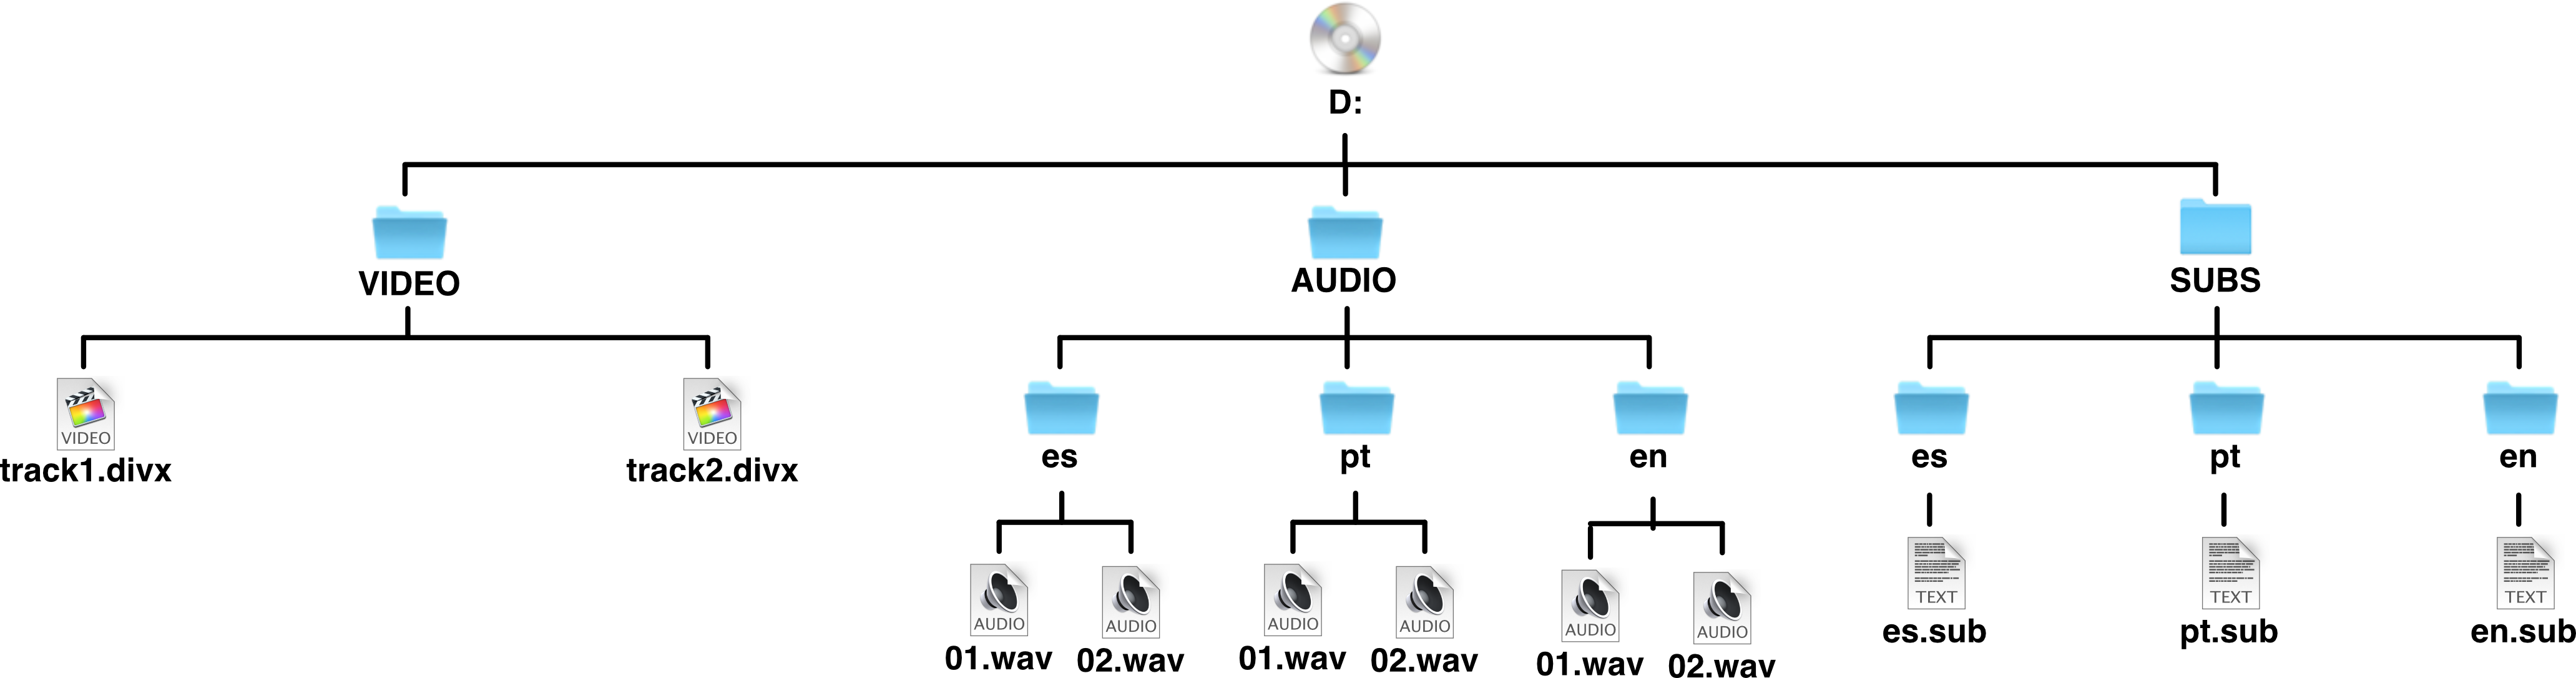
\includegraphics[scale=0.4]{capitulos/informatica/imagenes/directorios_windows_4.png}}

Se pide que escriba las siguientes rutas absolutas:
\begin{enumerate}[a)]
    \item Al archivo de subtítulos en inglés (en.sub)
    \item Al archivo de audio de la pista 02 en español (carpeta es, archivo 02.wav)
    \item Al archivo de video de la pista 01 (track1.divx)
    \item Al archivo de audio de la pista 01 en portugués.
\end{enumerate}
\end{exercise}

\begin{exercise}
Teniendo en cuenta el sistema de directorios del ejercicio anterior y
sabiendo qué:
\begin{itemize}
    \item Todo archivo de subtítulos pesa 500 KB.
    \item Los archivos de audio de la pista 01 pesan 5 MB.
    \item Los archivos de audio de la pista 02 pesan 25 MB, menos el de idioma
        portugués que pesa 27 MB.
    \item El archivo de video de la pista 01 pesa 340 MB
    \item El archivo de video de la pista 02 pesa 660 MB.
\end{itemize}

Se pide determine las siguientes:
\begin{enumerate}[a)]
    \item Cuanto pesa la carpeta VIDEO
    \item Cuanto pesa la carpeta SUBS
    \item Cuanto pesa en total el disco D:
\end{enumerate}
\end{exercise}

\begin{exercise}
Teniendo en cuenta la siguiente porción de un sistema de archivos de un
sistema Linux:

\centerline{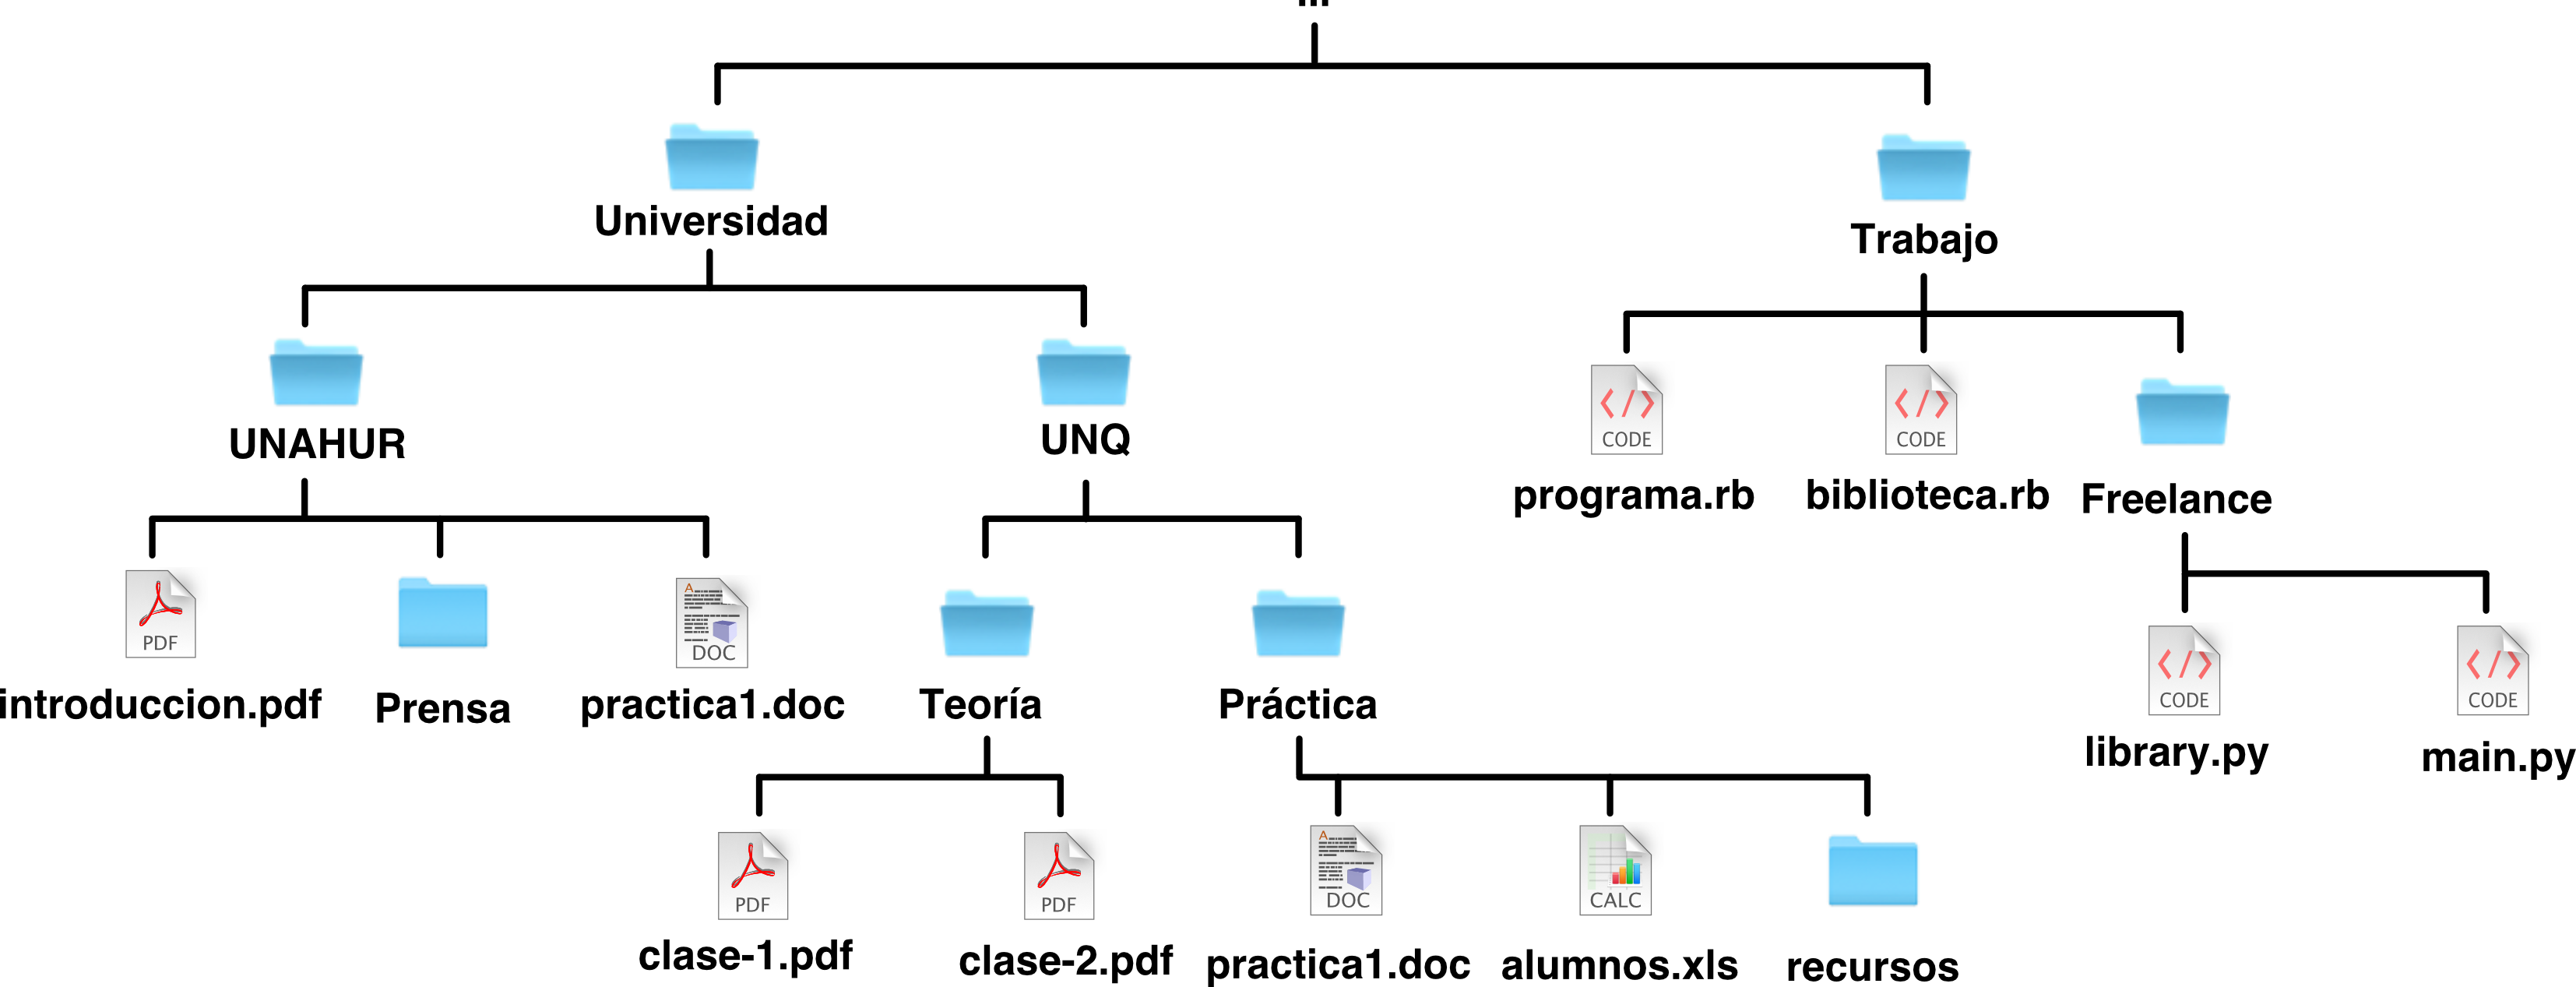
\includegraphics[scale=0.4]{capitulos/informatica/imagenes/directorios_relativos.png}}

Describa la ruta absoluta a las carpetas que se encuentren vacías, asumiendo que la
carpeta superior es la raíz del sistema.
\end{exercise}

\begin{exercise}
Utilizando el mismo sistema de archivos del ejercicio anterior, escriba
las siguientes rutas relativas:
\begin{enumerate}[a)]
    \item Desde la carpeta más externa de la jerarquía hasta el archivo
        main.py
    \item Desde la carpeta más externa de la jerarquía hasta el archivo
        alumnos.xls
    \item Desde la carpeta UNQ hasta el archivo clase-2.pdf
    \item Desde la carpeta UNAHUR al archivo introducción.pdf
    \item Desde la carpeta UNQ al archivo introducción.pdf
    \item Desde la carpeta Teoría en UNQ al archivo programa.rb
\end{enumerate}
\end{exercise}


\begin{exercise}
Un programa ``hola mundo'' consiste en código que simplemente imprime en la
pantalla las palabras ``hola mundo''. Este tipo de programa se ha hecho popular
como una forma de poder dar a los programadores una vista mínima y rápida de
la sintaxis de un lenguaje, y en cursos que se enfocan en la enseñanza de lenguajes
de programación en lugar de sus conceptos, es muy común encontrarlo como una de
las primeras muestras de código o actividades a realizar.

Se pide entonces que busque en internet el código de un programa ``hola mundo''
para los siguientes lenguajes de programación. Puede encontrar una gran colección
en el sitio \href{http://helloworldcollection.de}{http://helloworldcollection.de}

\begin{enumerate}[a)]
    \item Python
    \item Lisp
    \item C
    \item Java
    \item Assembly ARM
    \item Assembly z80, Console
\end{enumerate}

¿Qué reflexiones puede realizar después de ver los diferentes códigos?
\end{exercise}

\begin{exercise}
El sitio web \href{https://alternativeto.net}{https://alternativeto.net} permite
a sus usuarios buscar un programa por nombre, y brinda alternativas a ese programa
con funcionalidades equivalentes o similares. Dentro de los resultados, se puede
filtrar por sistema operativo y por el tipo de licencia (comercial, gratuita o libre).

Se pide que busque al menos una alternativa que sea software libre y/o open
source para cada uno de los siguientes programas:
\begin{enumerate}[a)]
    \item Windows 10
    \item Microsoft Office Suite
    \item Adobe Acrobat Reader
    \item Internet Explorer
    \item Adobe Photoshop
    \item Autodesk AutoCAD
    \item Age of Empires II
\end{enumerate}
\end{exercise}